\documentclass[11pt]{article}
\usepackage{amsthm}
\usepackage{amssymb}
\usepackage{enumitem}
\usepackage{amsmath, physics}
\usepackage{bm}
\usepackage{adjustbox}
\usepackage{mathrsfs}
\usepackage{graphicx}
\usepackage{siunitx}
\usepackage[mathscr]{euscript}

\title{\textbf{Solved selected problems of Modern Physics for Scientists and Engineers - John Taylor}}
\author{Franco Zacco}
\date{}

\addtolength{\topmargin}{-3cm}
\addtolength{\textheight}{3cm}

\newcommand{\N}{\mathbb{N}}
\newcommand{\Z}{\mathbb{Z}}
\newcommand{\Q}{\mathbb{Q}}
\newcommand{\R}{\mathbb{R}}
\newcommand{\diam}{\text{diam}}
\newcommand{\cl}{\text{cl}}
\newcommand{\bdry}{\text{bdry}}
\newcommand{\inter}{\text{int}}
\newcommand{\hatx}{\bm{\hat{x}}}
\newcommand{\haty}{\bm{\hat{y}}}
\newcommand{\hatz}{\bm{\hat{z}}}
\newcommand{\hatrho}{\bm{\hat{\rho}}}
\newcommand{\hatphi}{\bm{\hat{\phi}}}
\newcommand{\hatr}{\bm{\hat{r}}}
\newcommand{\hattheta}{\bm{\hat{\theta}}}
\newcommand{\sci}[1]{\times 10^{#1}}
\newcommand{\expect}[1]{\left\langle {#1} \right\rangle}

\theoremstyle{definition}
\newtheorem*{solution*}{Solution}
\renewcommand*{\proofname}{\bf{Solution}}

\begin{document}
\maketitle
\thispagestyle{empty}

\section*{Chapter 8 - The Three-Dimensional Schrödinger Equation}

\begin{proof}{\textbf{8.4}}
For a free particle subject to no forces, equation (8.2) becomes
\begin{align*}
    \pdv[2]{\psi}{x} + \pdv[2]{\psi}{y} + \pdv[2]{\psi}{z}
    = -\frac{2M}{\hbar^2}E\psi
\end{align*}
We want to show that $\psi(\bm{r}) = e^{i\bm{k\cdot r}}$ is a solution for any
fixed vector $\bm{k}$ satisfying $E = \hbar^2 \bm{k}^2/2M$ hence we replace
$\psi$ and $E$ and we solve the equation
\begin{align*}
    -k_x^2e^{i\bm{k\cdot r}} - k_y^2e^{i\bm{k\cdot r}} - k_z^2e^{i\bm{k\cdot r}}
    &= -\frac{2M}{\hbar^2}\frac{\hbar^2\bm{k}^2}{2M} e^{i\bm{k\cdot r}}\\
    -e^{i\bm{k\cdot r}}(k_x^2 + k_y^2 + k_z^2)
    &= -\bm{k}^2 e^{i\bm{k\cdot r}}\\
    k_x^2 + k_y^2 + k_z^2 &= \bm{k}^2
\end{align*}
Where $k_x, k_y$ and $k_z$ are the components of the vector $\bm{k}$.
We see that the equality holds, so $\psi(\bm{r}) = e^{i\bm{k\cdot r}}$
is a solution to the three-dimensional Schrödinger equation.
\\
The vector $\bm{k}$ can be viewed as the angular frequency vector, where each
component represents the angular frequency of the wave equation in a particular
direction.
\end{proof}

\cleardoublepage
\begin{proof}{\textbf{8.8}}
\begin{center}
    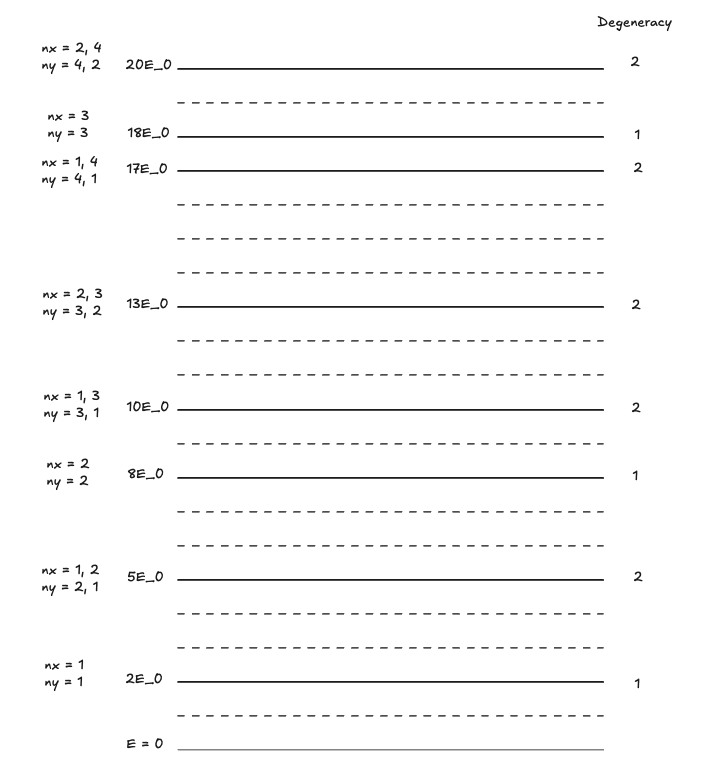
\includegraphics[scale=0.55]{ch8-8.8.png}
\end{center}
\end{proof}

\cleardoublepage
\begin{proof}{\textbf{8.9}}
Consider a particle of mass $M$ in a two-dimensional, rigid rectangular box
with sides $a$ and $b$. Following the same steps as in Section 8.3 from
equation (8.3) to equation (8.15) everything in between applies to this case.
We arrive to the following differential equations
\begin{align*}
    X''(x) &= -k_x^2 X(x)\qquad
    Y''(y) = -k_y^2 Y(y)
\end{align*}
For which we know the solutions are
\begin{align*}
    X(x) &= B\sin k_x x\qquad
    Y(y) = C\sin k_y y
\end{align*}
And to satisfy the boundary conditions $X(x) = 0$ at $x = 0\text{ or }a$ and
$Y(y) = 0$ at $y=0 \text{ or } b$ we need that
\begin{align*}
    k_x = \frac{n_x\pi}{a}\qquad
    k_y = \frac{n_y\pi}{b}
\end{align*}
Now combining the solutions we get the complete wave function solution
\begin{align*}
    \psi(x,y) &= A\sin(\frac{n_x \pi x}{a})\sin(\frac{n_y \pi y}{b})
\end{align*}
Where we renamed the constant $BC$ as $A$.
\\
On the other hand, from equation (8.10) we know that
\begin{align*}
    \frac{X''(x)}{X(x)} + \frac{Y''(y)}{Y(y)} = -\frac{2ME}{\hbar^2}
\end{align*}
But $X''(x)/X(x) = -k_x^2$ and $Y''(y)/Y(y) = -k_y^2$ then
\begin{align*}
    -\frac{2ME}{\hbar^2} &= -\frac{n_x^2\pi^2}{a^2} -\frac{n_y^2\pi^2}{b^2}\\
    E_{n_x, n_y}
    &= \frac{\pi^2\hbar^2}{2M}\bigg(\frac{n_x^2}{a^2} + \frac{n_y^2}{b^2}\bigg)
\end{align*}
Which gives us the allowed energies.
\end{proof}

\cleardoublepage
\begin{proof}{\textbf{8.10}}
Let
$$E_0 = \frac{\hbar^2\pi^2}{2Ma^2}$$
Then equation (8.102) for the case $b = a/2$ becomes
\begin{align*}
    E_{n_x,n_y} = E_0(n_x^2 + 4n_y^2)
\end{align*}
Then the six lowest energy levels, with their quantum numbers and degeneracies
are
\begin{align*}
    E_{n_x, n_y} & &\text{Degeneracy}& &n_x, n_y\\
    5E_0&  &1&  &\begin{cases} n_x = 1\\ n_y = 1 \end{cases}\\
    8E_0&  &1&  &\begin{cases} n_x = 2\\ n_y = 1 \end{cases}\\
    13E_0&  &1&  &\begin{cases} n_x = 3\\ n_y = 1 \end{cases}\\
    17E_0&  &1&  &\begin{cases} n_x = 1\\ n_y = 2 \end{cases}\\
    20E_0&  &2&  &\begin{cases} n_x = 2,4\\ n_y = 2,1 \end{cases}\\
    25E_0&  &1&  &\begin{cases} n_x = 3\\ n_y = 2 \end{cases}   
\end{align*}
\end{proof}

\cleardoublepage
\begin{proof}{\textbf{8.11}}
Let $a = 1.1b$ then the equation (8.102) for this case becomes
\begin{align*}
    E_{n_x,n_y} = E_0\bigg(\frac{n_x^2}{(1.1)^2} + n_y^2\bigg)
\end{align*}
Then the six lowest energy levels, with their quantum numbers and degeneracies
are
\begin{align*}
    E_{n_x, n_y} & &\text{Degeneracy}& &n_x, n_y\\
    1.82E_0&  &1&  &\begin{cases} n_x = 1\\ n_y = 1 \end{cases}\\
    4.3E_0&  &1&  &\begin{cases} n_x = 2\\ n_y = 1 \end{cases}\\
    4.82E_0&  &1&  &\begin{cases} n_x = 1\\ n_y = 2 \end{cases}\\
    7.3E_0&  &1&  &\begin{cases} n_x = 2\\ n_y = 2 \end{cases}\\
    8.43E_0&  &1&  &\begin{cases} n_x = 3\\ n_y = 1 \end{cases}\\
    9.82E_0&  &1&  &\begin{cases} n_x = 1\\ n_y = 3 \end{cases}   
\end{align*}
We see that the degeneracies $n_x = 1,2, n_y = 2,1$ and $n_x = 3,1, n_y = 1,3$
disappear.
\end{proof}

\cleardoublepage
\begin{proof}{\textbf{8.12}}
\begin{itemize}
\item [\textbf{(a)}] Let $n_x = 1$ and $n_y = 2$ then
\begin{align*}
    |\psi(x,y)|^2 = A^2\sin^2\frac{\pi x}{a}\sin^2\frac{2\pi y}{a}
\end{align*}
Then the maximum of $|\psi|^2$ happen at $x = a/2$ and $y = a/4, 3a/4$
so we have 2 points where the particle is most likely to be found.
Below we show the contour map for this case
\begin{center}
    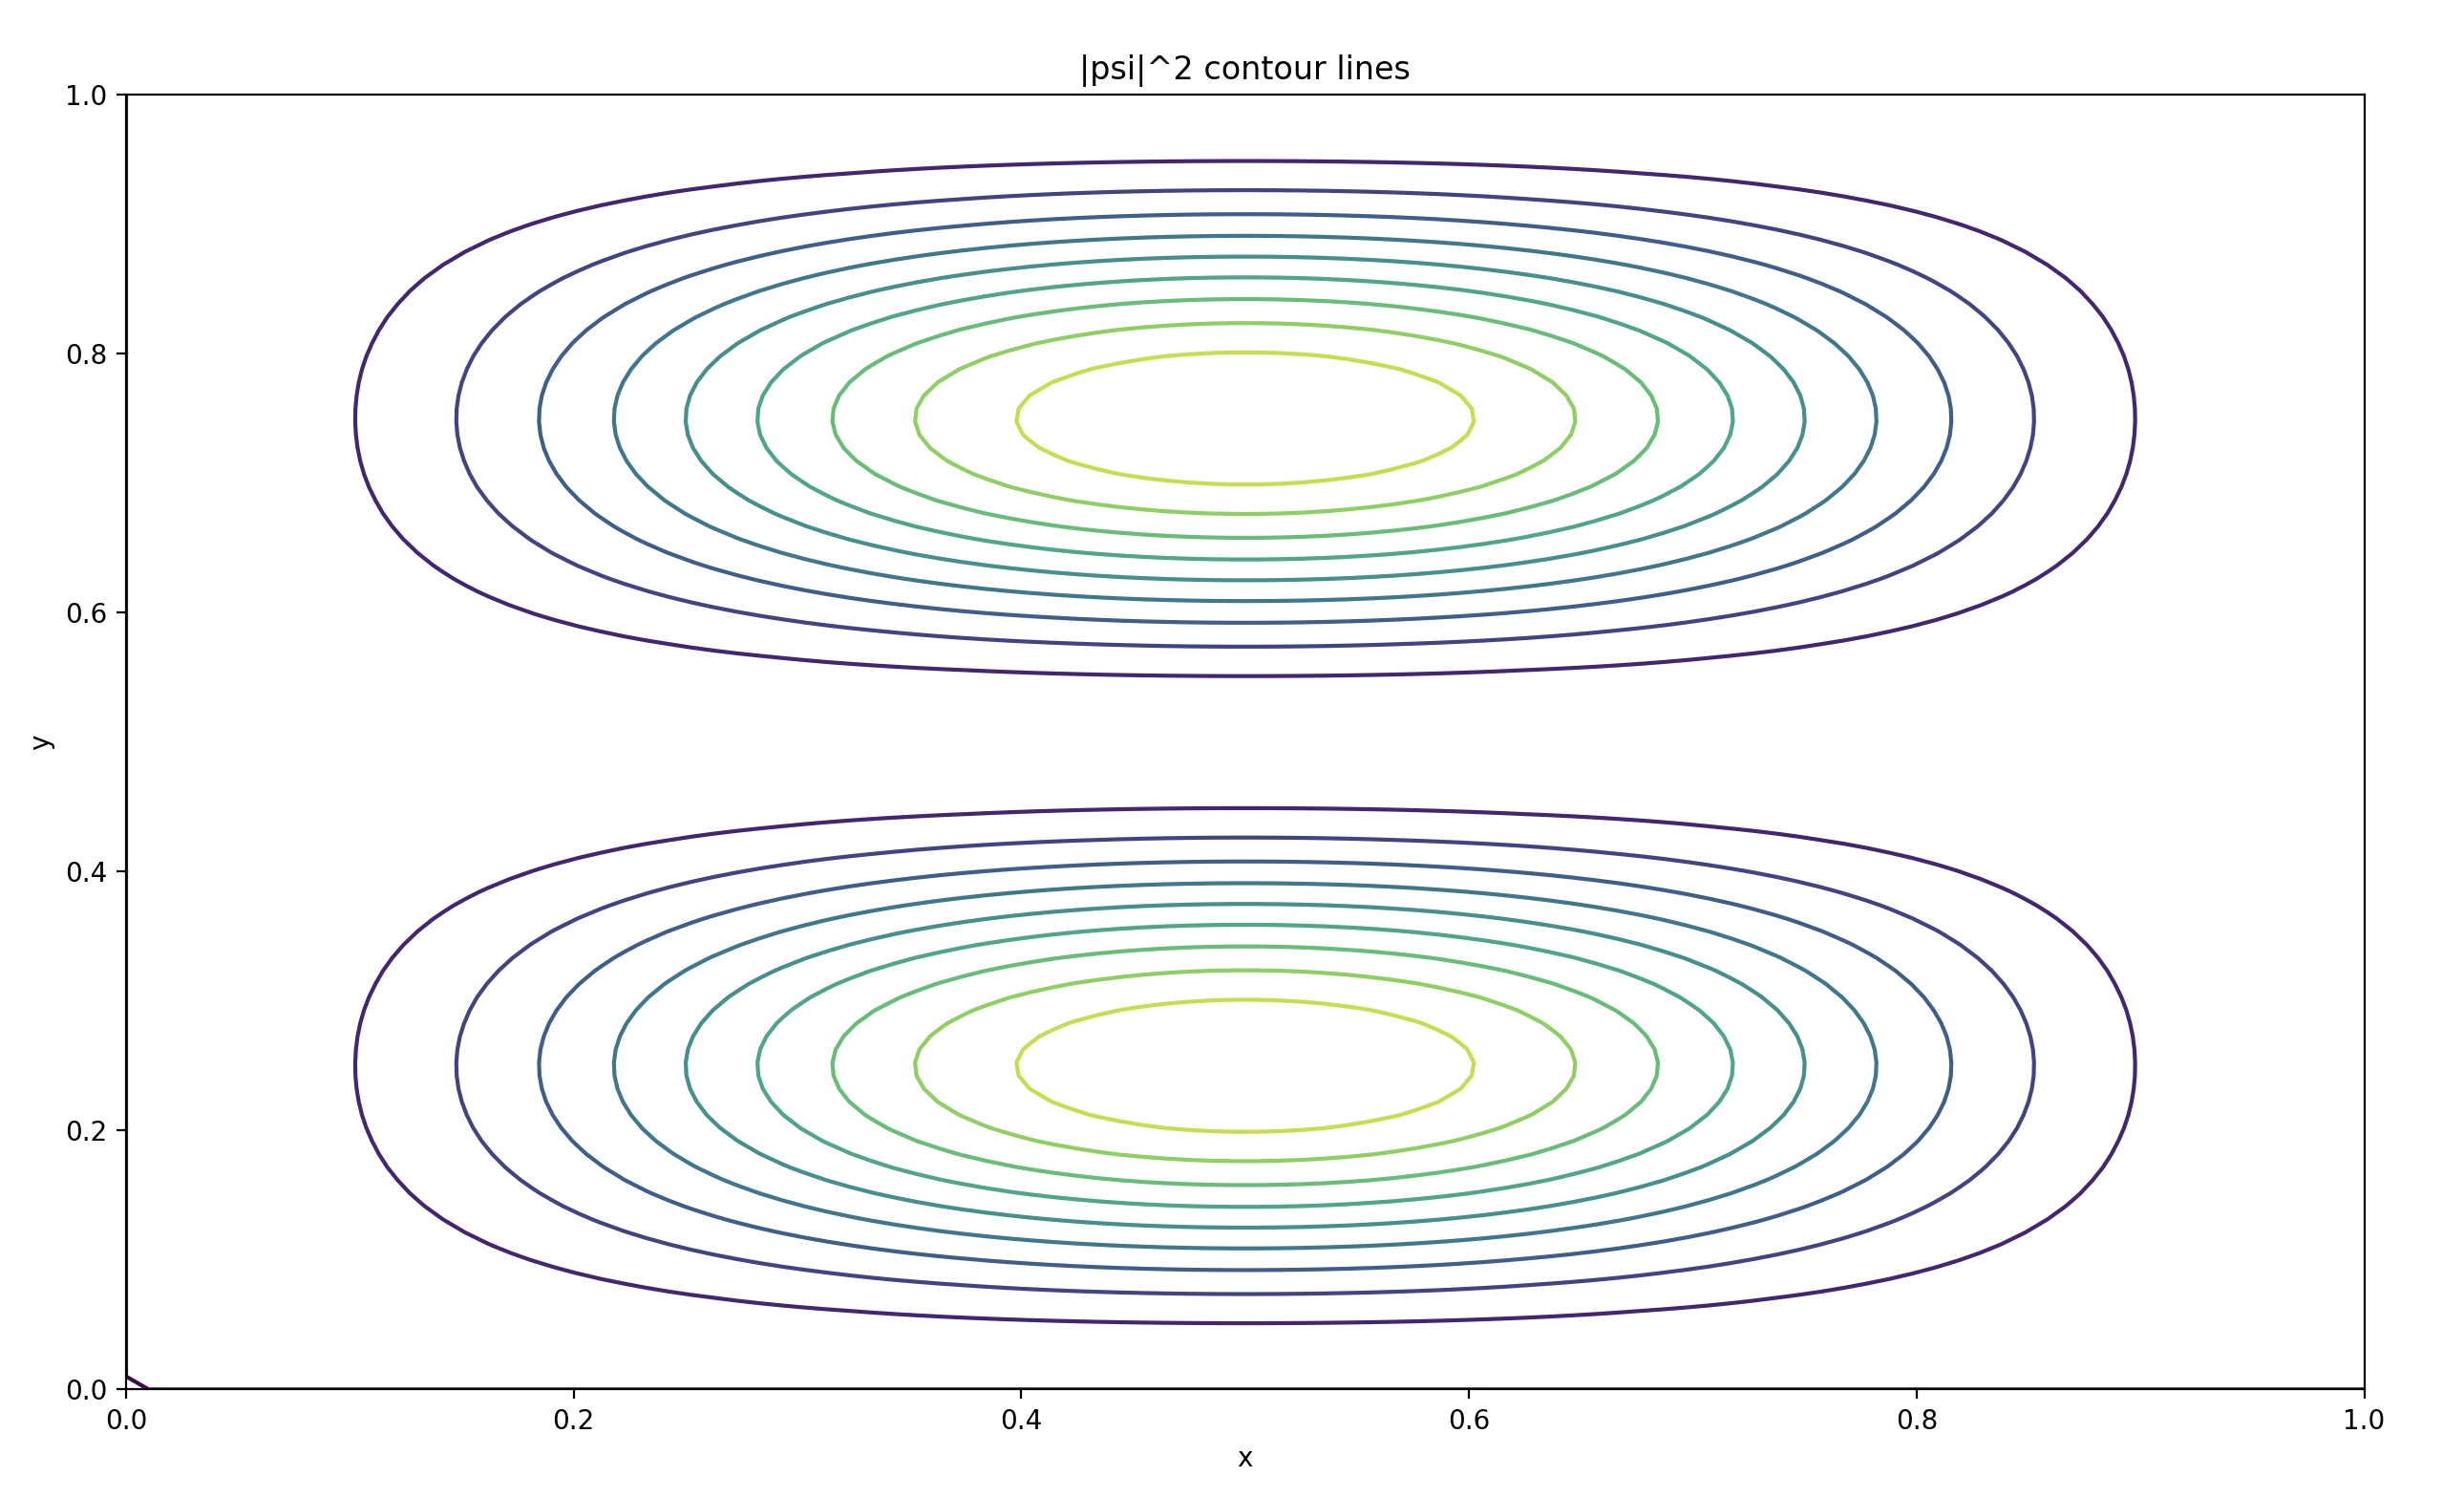
\includegraphics[scale=0.25]{ch8-8.12a.png}
\end{center}
\item [\textbf{(b)}] Let $n_x = 2$ and $n_y = 2$ then the contour map looks
like
\begin{center}
    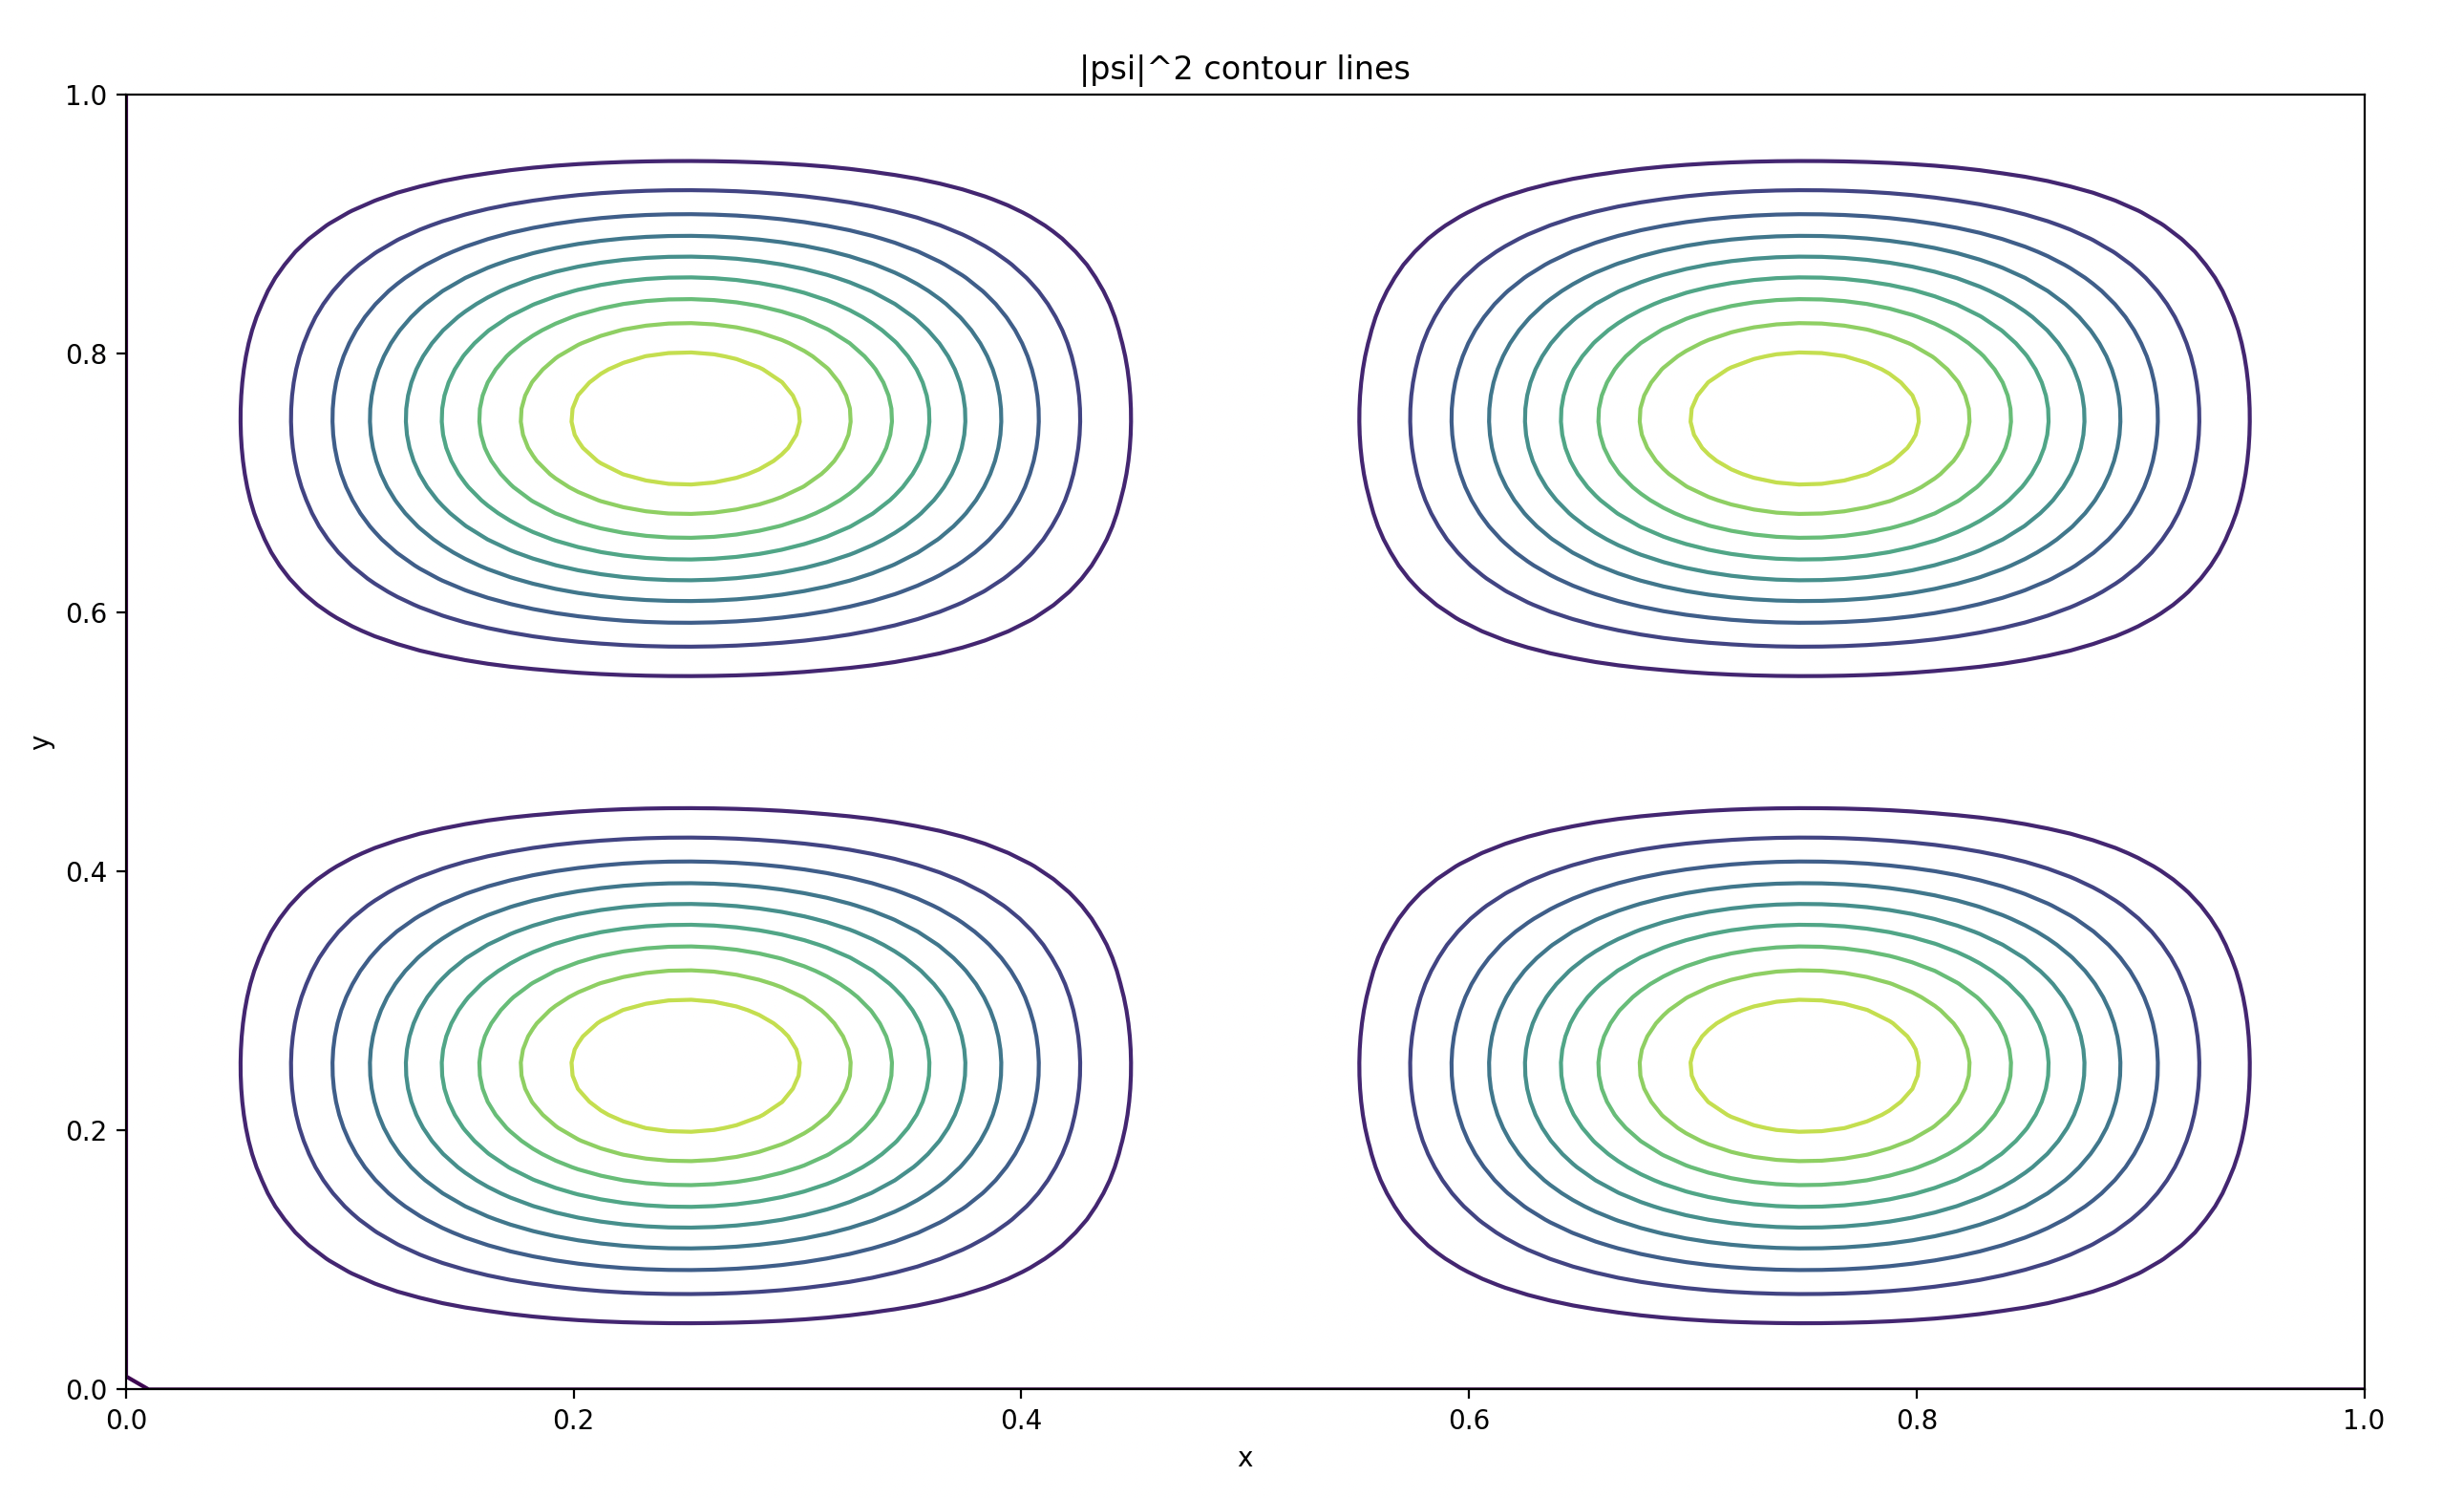
\includegraphics[scale=0.25]{ch8-8.12b.png}
\end{center}

\cleardoublepage
\item [\textbf{(c)}] Let $n_x = 4$ and $n_y = 3$ then the contour map looks
like
\begin{center}
    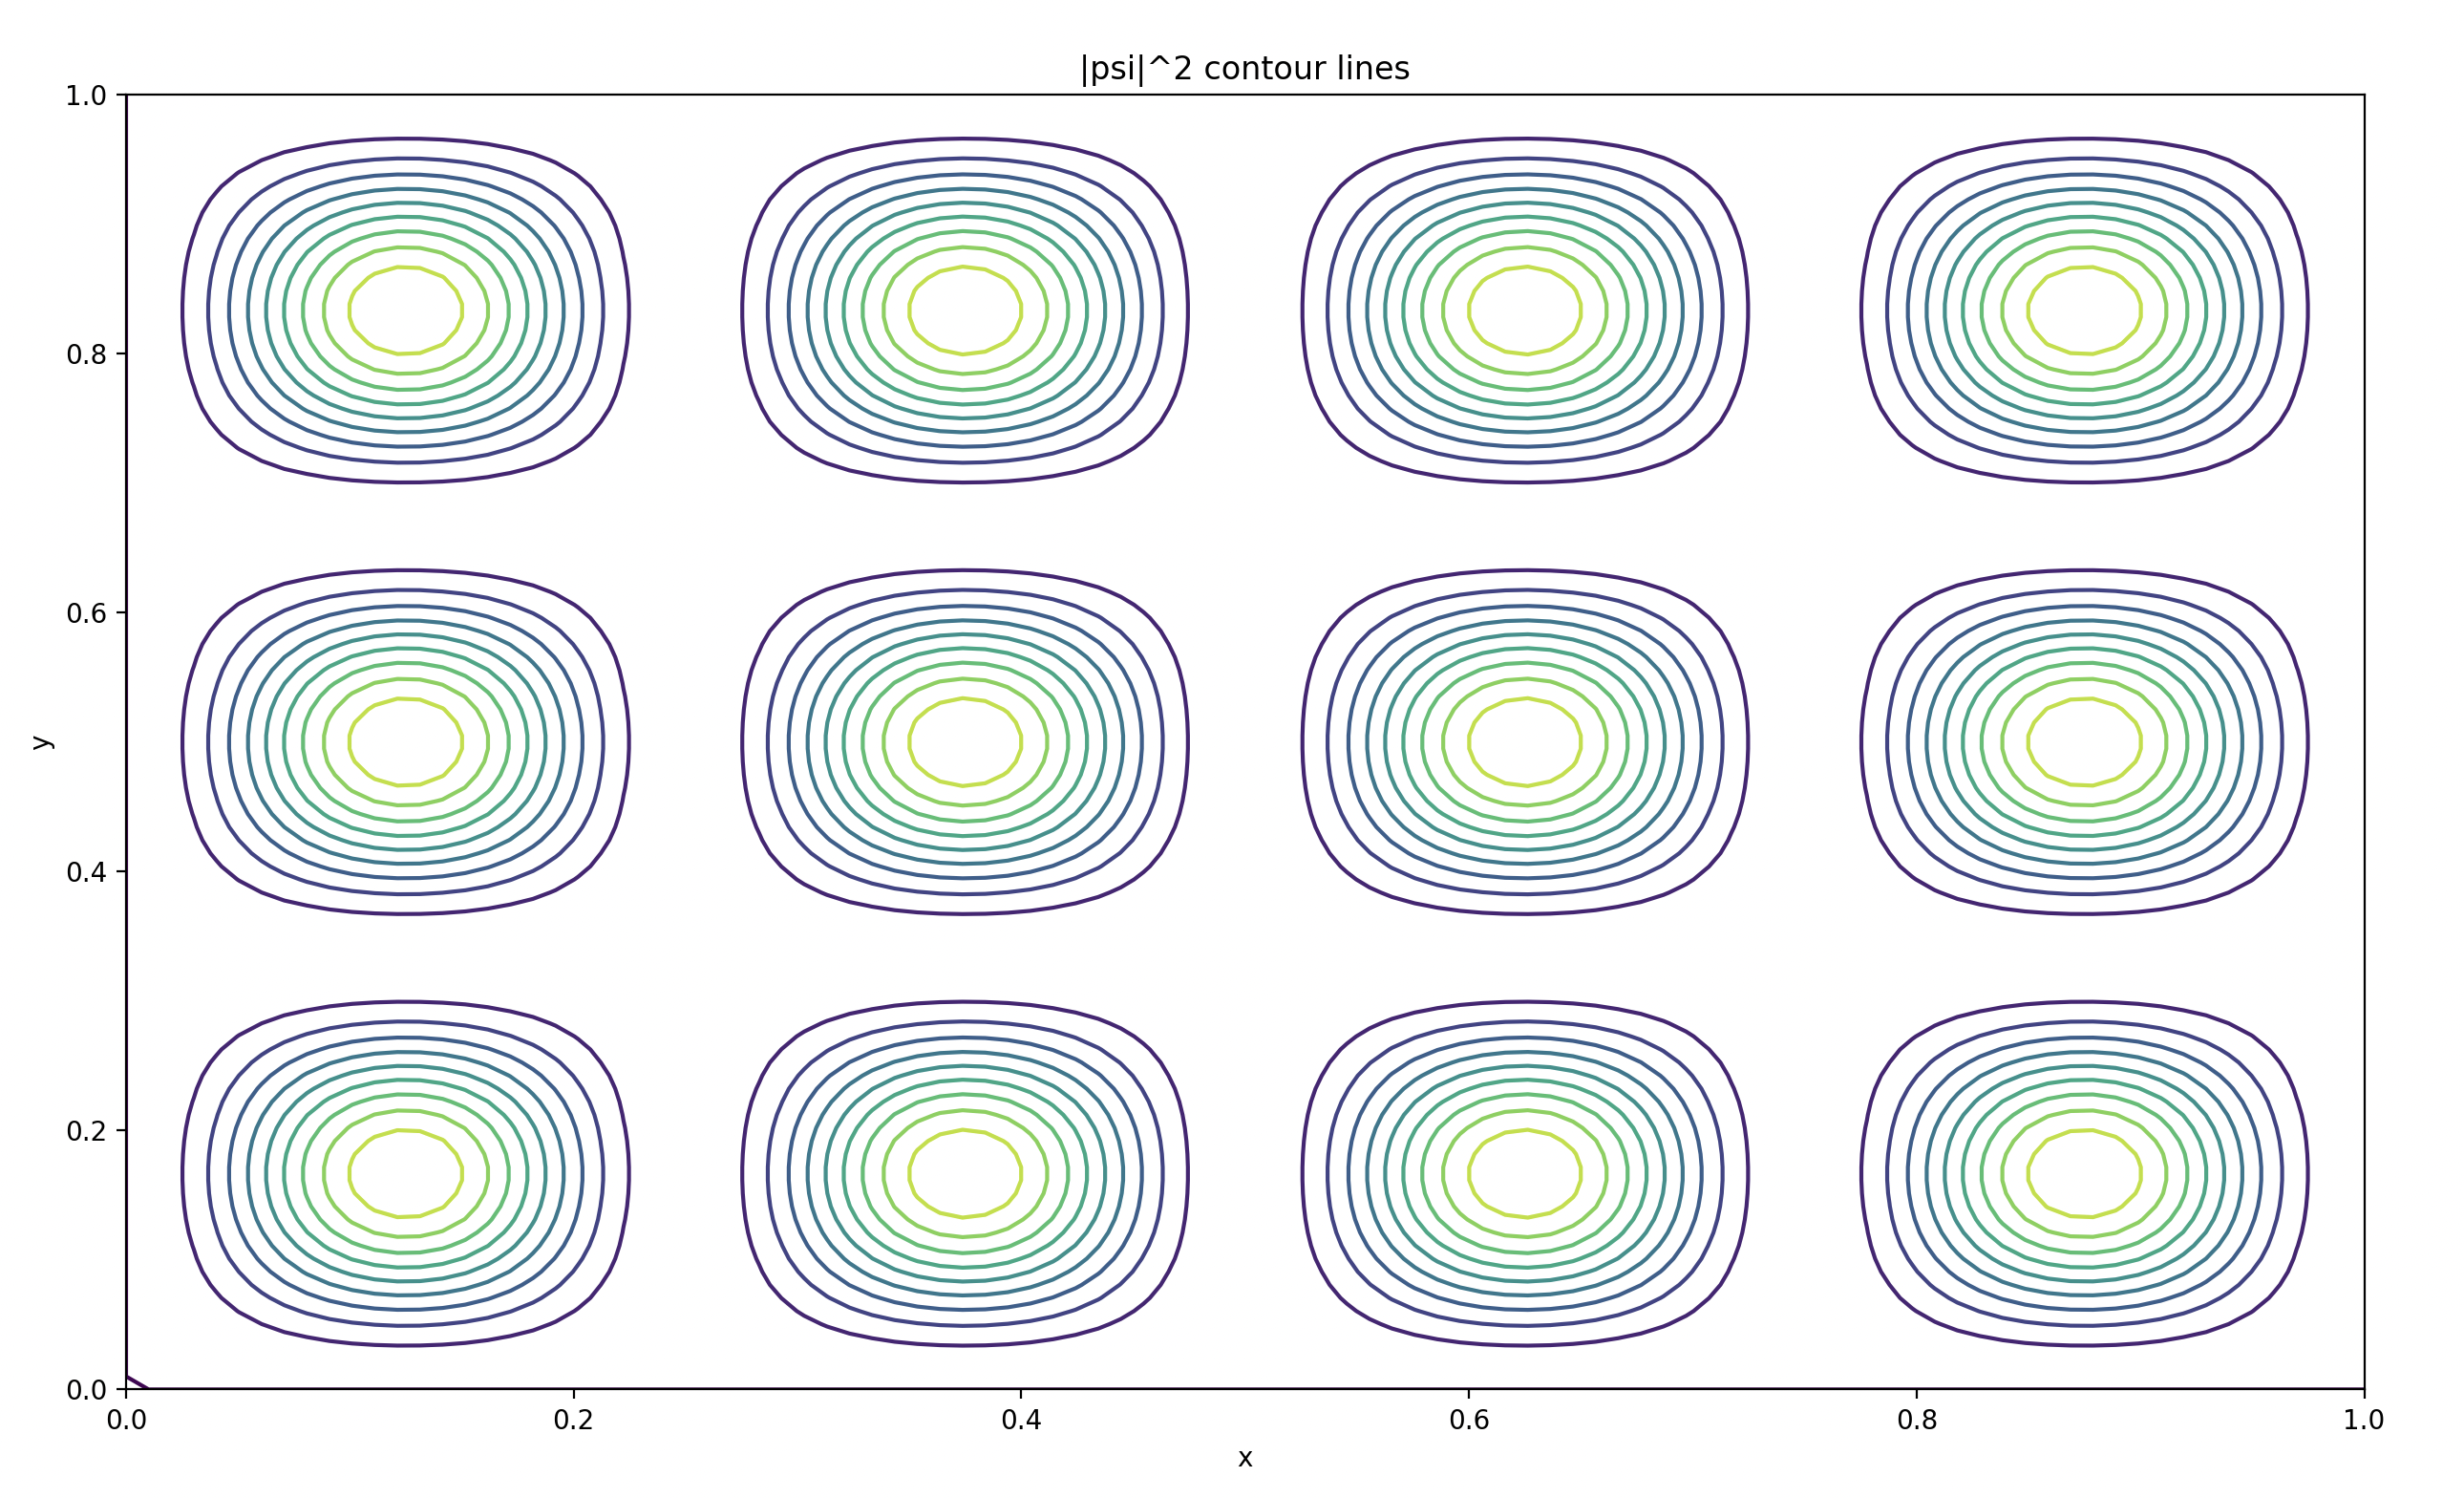
\includegraphics[scale=0.25]{ch8-8.12c.png}
\end{center}

\end{itemize}
\end{proof}

\cleardoublepage
\begin{proof}{\textbf{8.22}}
\begin{itemize}
\item [\textbf{(a)}] Let $\psi = R(r)\Theta(\theta)\Phi(\phi)$, then, replacing
in the Schrödinger equation for spherical coordinates we get that
\begin{align*}
    &\frac{\Theta\Phi}{r}\pdv[2]{r}(rR)
    + \frac{R\Phi}{r^2\sin\theta}\pdv{\theta}(\sin\theta\pdv{\Theta}{\theta})
    + \frac{R\Theta}{r^2\sin^2\theta}\pdv[2]{\Phi}{\phi} = \\
    &\qquad= \frac{2M}{\hbar^2}[U(r) - E]R\Theta\Phi
\end{align*}
Multiplying the equation by $r^2\sin^2\theta/(R\Theta\Phi)$ we have that
\begin{align*}
    &\frac{r\sin^2\theta}{R}\pdv[2]{r}(rR)
    + \frac{\sin\theta}{\Theta}\pdv{\theta}(\sin\theta\pdv{\Theta}{\theta})
    + \frac{1}{\Phi}\pdv[2]{\Phi}{\phi} = \\
    &\qquad= \frac{2M}{\hbar^2}[U(r) - E]r^2\sin^2\theta
\end{align*}
Rearranging
\begin{align*}
    \frac{1}{\Phi}\pdv[2]{\Phi}{\phi}
    = \frac{2M}{\hbar^2}[U(r) - E]r^2\sin^2\theta
    - \frac{r\sin^2\theta}{R}\pdv[2]{r}(rR)
    - \frac{\sin\theta}{\Theta}\pdv{\theta}(\sin\theta\pdv{\Theta}{\theta})
\end{align*}
So we got
\begin{align*}
    \frac{\Phi''(\phi)}{\Phi(\phi)} = \text{function of $r$ and $\theta$}
\end{align*}
Since the RHS is independent of $\phi$ and the LHS is independent of $r$ and
$\theta$ they must be equal to a constant, otherwise a change in the LHS
would imply a change in the RHS to maintain the equality, which doesn't make
sense since they are independent.
\\
Naming the constant $-m^2$ gives us
\begin{align*}
    \Phi''(\phi) = -m^2\Phi(\phi)
\end{align*}

\item [\textbf{(b)}] On the other hand, this implies that
\begin{align*}
    \frac{2M}{\hbar^2}[U(r) - E]r^2\sin^2\theta
    - \frac{r\sin^2\theta}{R}\pdv[2]{r}(rR)
    - \frac{\sin\theta}{\Theta}\pdv{\theta}(\sin\theta\pdv{\Theta}{\theta})
    = -m^2
\end{align*}
Multiplying the equation by $1/\sin^2\theta$ gives us
\begin{align*}
    \frac{2M}{\hbar^2}[U(r) - E]r^2
    - \frac{r}{R}\pdv[2]{r}(rR)
    - \frac{1}{\Theta\sin\theta}\pdv{\theta}(\sin\theta\pdv{\Theta}{\theta})
    = -\frac{m^2}{\sin^2\theta}
\end{align*}
And rearranging it we get
\begin{align*}
    \frac{1}{\Theta\sin\theta}\pdv{\theta}(\sin\theta\pdv{\Theta}{\theta})
    -\frac{m^2}{\sin^2\theta}
    &= \frac{2M}{\hbar^2}[U(r) - E]r^2 - \frac{r}{R}\pdv[2]{r}(rR)
\end{align*}
Again, since the LHS is independent of $r$ and the RHS is independent of
$\theta$, then each side must be equal to a constant. Let us call the constant
$-k$, then the LHS give us
\begin{align*}
    \frac{1}{\Theta\sin\theta}\pdv{\theta}(\sin\theta\pdv{\Theta}{\theta})
    -\frac{m^2}{\sin^2\theta} &= -k\\
    \frac{1}{\sin\theta}\pdv{\theta}(\sin\theta\pdv{\Theta}{\theta})
    + \bigg(k-\frac{m^2}{\sin^2\theta}\bigg)\Theta &= 0
\end{align*}
Finally, the RHS is
\begin{align*}
    \frac{2M}{\hbar^2}[U(r) - E]r^2 - \frac{r}{R}\pdv[2]{r}(rR) &= -k\\
    \frac{r}{R}\pdv[2]{r}(rR) &= k + \frac{2M}{\hbar^2}[U(r) - E]r^2\\
    \frac{r}{R}\pdv[2]{r}(rR)
    &= \frac{2M}{\hbar^2}\bigg[\frac{k\hbar^2}{2M} + [U(r) - E]r^2\bigg]\\
    \pdv[2]{r}(rR)
    &= \frac{2M}{\hbar^2}\bigg[\frac{k\hbar^2}{2Mr^2} + U(r) - E\bigg]rR
\end{align*}
\end{itemize}
\end{proof}

\cleardoublepage
\begin{proof}{\textbf{8.23}}
The minimum possible angle between $\bm L$ and the z axis in the case $l = 2$
happens for $m = 2$ hence $L_z = 2\hbar$ so
\begin{align*}
    \theta = \arccos(\frac{2\hbar}{\sqrt{2(2 + 1)}\hbar})
    = 0.6154~\text{rad} = 35.26^\circ
\end{align*}
\end{proof}
\begin{proof}{\textbf{8.24}}
\begin{itemize}
\item [\textbf{(a)}] Angular momentum when $l= 1$.
\begin{center}
    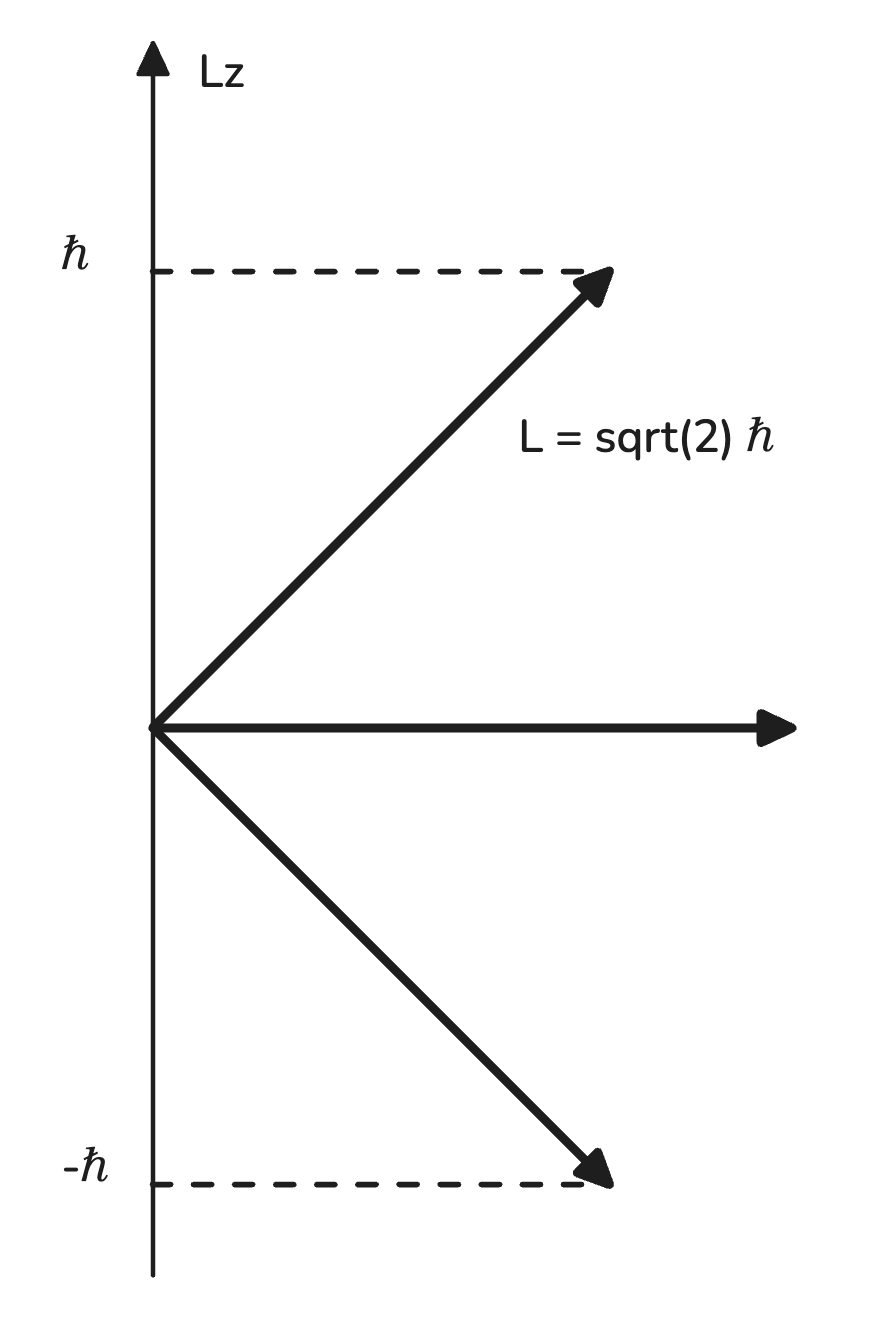
\includegraphics[scale=0.3]{ch8_8.24.png}
\end{center}
\item [\textbf{(b)}] There are $(2l + 1) = 3$ possible orientations
\item [\textbf{(c)}] The minimum possible angle between $\bm L$ and the z axis
in the case $l = 1$ happens for $m = 1$ hence $L_z = \hbar$ so
\begin{align*}
    \theta = \arccos(\frac{1\hbar}{\sqrt{1(1 + 1)}\hbar})
    = 0.7853~\text{rad} = 45^\circ
\end{align*}
\end{itemize}
\end{proof}

\cleardoublepage
\begin{proof}{\textbf{8.26}}
Given that the magnitude of $\bm{L}$ is $L = \sqrt{l(l +1 )} \hbar$ then by
definition $L_z$ is given by $L_z = m\hbar$ where $m$ can take values
$-l, -l+1, ..., l-1, l$, so the biggest magnitude $L_z$ can have is
$L_z = l\hbar$.
\\
We see that $l^2 \leq l^2 + l$ then $l \leq \sqrt{l(l+1)}$. Therefore the
largest value of $L_z$ is less than or equal to $L$.
\end{proof}
\begin{proof}{\textbf{8.27}}
The ratios $L/L_{bohr}$ are
\begin{align*}
l &= 1 & \frac{L}{L_{bohr}} &= \frac{\sqrt{1(1 + 1)}\hbar}{1 \hbar} = 1.414\\
l &= 2 & \frac{L}{L_{bohr}} &= \frac{\sqrt{2(2 + 1)}\hbar}{2 \hbar} = 1.224\\
l &= 3 & \frac{L}{L_{bohr}} &= \frac{\sqrt{3(3 + 1)}\hbar}{3 \hbar} = 1.154\\
l &= 4 & \frac{L}{L_{bohr}} &= \frac{\sqrt{4(4 + 1)}\hbar}{4 \hbar} = 1.118\\
l &= 10 & \frac{L}{L_{bohr}} &= \frac{\sqrt{10(10 + 1)}\hbar}{10 \hbar} = 1.048\\
l &= 100 & \frac{L}{L_{bohr}} &= \frac{\sqrt{100(100 + 1)}\hbar}{100 \hbar} = 1.004
\end{align*}
We see that as $l$ grows then $L/L_{bohr}$ tends to 1 which implies that for
big $l$ then $L_{bohr}$ is quite close to the correct $L$.

\end{proof}
\begin{proof}{\textbf{8.28}}
The allowed magnitudes of the angular momentum are 
\begin{align*}
    L = \sqrt{l(l + 1)}\hbar = \sqrt{l^2\bigg(1 + \frac{1}{l}\bigg)}\hbar
    = l\sqrt{1 + \frac{1}{l}}\hbar
\end{align*}
If $l$ is large then we can approximate the square root using the binomial
expansion as follows
\begin{align*}
    L \approx l\bigg(1 + \frac{1}{2l}\bigg)\hbar
    = \bigg(l + \frac{1}{2}\bigg)\hbar
\end{align*}
\end{proof}

\cleardoublepage
\begin{proof}{\textbf{8.29}}
The equation for $\theta$ when $m = l = 0$ becomes
\begin{align*}
    \dv{\theta}(\sin\theta\dv{\Theta}{\theta}) = 0
\end{align*}
\begin{itemize}
\item [\textbf{(a)}] Let $\Theta = C$ where $C$ is a constant then
$d\Theta/d\theta = d(C)/d\theta = 0$ so the equation is satisfied.
\item [\textbf{(b)}] Let
\begin{align*}
    \Theta = \ln(\frac{1 + \cos\theta}{1 - \cos\theta})
\end{align*}
Then
\begin{align*}
    \dv{\Theta}{\theta} = -\frac{2}{\sin\theta}
\end{align*}
Hence 
\begin{align*}
    \dv{\theta}(\sin\theta\dv{\Theta}{\theta}) = \dv{\theta}(-2) = 0
\end{align*}
So the function $\Theta$ is a solution of the $\theta$ equation.

If we let $\theta = 0$ we see that
\begin{align*}
    \Theta = \ln(\frac{1 + 1}{1 - 1}) \to \infty
\end{align*}
and if we let $\theta = \pi$ we get that
\begin{align*}
    \Theta = \ln(\frac{1 + (-1)}{1 - (-1)}) \to -\infty
\end{align*}
Since $\lim_{x\to \infty} \ln(x) = \infty$ and $\lim_{x\to 0} \ln(x) = -\infty$.

\item [\textbf{(c)}]
Then the general solution for the $\theta$ equation must be a linear combination
of both solutions 
\begin{align*}
    \Theta = aC + b\ln(\frac{1 + \cos\theta}{1 - \cos\theta})
\end{align*}
where $a, b$ are constants. Again for $\theta = 0$ or $\pi$ we get that
$\Theta \to \infty$ or $\Theta \to -\infty$ respectively, so the second term
cannot be part of the general solution since it's not well defined for every
$\theta$. Therefore only the solution $\Theta = C$ is an acceptable solution.
\end{itemize}
\end{proof}

\cleardoublepage
\begin{proof}{\textbf{8.30}}
The $\theta$ equation for the case $l = m = 1$ is
\begin{align*}
    \frac{1}{\sin\theta}\dv{\theta}(\sin\theta \dv{\Theta}{\theta})
    + \bigg(2 - \frac{1}{\sin^2\theta}\bigg)\Theta = 0
\end{align*}
Let $\Theta = \sin\theta$ then we see that
\begin{align*}
    &\frac{1}{\sin\theta}\dv{\theta}(\sin\theta \dv{\Theta}{\theta})
    + \bigg(2 - \frac{1}{\sin^2\theta}\bigg)\Theta =\\
    &\qquad=\frac{1}{\sin\theta}\dv{\theta}(\sin\theta \cos\theta)
    + \bigg(2 - \frac{1}{\sin^2\theta}\bigg)\sin\theta\\
    &\qquad=\frac{1}{\sin\theta}(\cos^2\theta - \sin^2\theta)
    + 2\sin\theta - \frac{1}{\sin\theta}\\
    &\qquad=\frac{\cos^2\theta}{\sin\theta}
    + \sin\theta - \frac{1}{\sin\theta}\\
    &\qquad=\frac{\cos^2\theta + \sin^2\theta - 1}{\sin\theta}\\
    &\qquad=\frac{1 - 1}{\sin\theta}\\
    &\qquad=0
\end{align*}
So $\Theta = \sin\theta$ is a solution of the $\theta$ equation.
\\
The complete wave functions for the cases $l = 1$, $m = 1$ and $l = 1$, $m = -1$
are 
\begin{align*}
    \psi(r, \theta, \phi) = R(r)\sin\theta e^{i\phi}
    \qquad
    \psi(r, \theta, \phi) = R(r)\sin\theta e^{-i\phi}
\end{align*}
Assuming $r$ fixed then $\psi$ only depends on $\theta$ and $\phi$ but
computing $|\psi|^2$ we see that
\begin{align*}
    |\psi|^2 \propto \sin^2\theta |e^{i\phi}|^2 = \sin^2\theta
\end{align*}
Since $|e^{i\phi}|^2 = 1$, then $|\psi|^2$ is maximum for $\theta = \pi/2$.
\\
In the case of $\psi(r, \theta, \phi) = R(r)\sin\theta e^{-i\phi}$ since
$|e^{-i\phi}|^2 = 1$ we get that $|\psi|^2$ is maximum for $\theta = \pi/2$
as well.


\end{proof}

\cleardoublepage
\begin{proof}{\textbf{8.31}}
Let $\Theta_{l,m}(\theta)$ be a solution to the $\theta$ equation
\begin{align*}
    \frac{1}{\sin\theta}\dv{\theta}(\sin\theta \dv{\Theta}{\theta})
    + \bigg(l(l + 1) - \frac{m^2}{\sin^2\theta}\bigg)\Theta = 0
\end{align*}
The $\theta$ equation for $l, -m$ is the same since it depends on
$(-m)^2 = m^2$, then the $\theta$ equation for $l, -m$ must
also be solved by $\Theta_{l,m}(\theta)$ but the $\theta$ equation has at most
one independent acceptable solution for any given values of $l$ and $m$, so
must be that the solution $\Theta_{l, -m}(\theta)$ is at most proportional to
$\Theta_{l, m}(\theta)$ i.e. $\Theta_{l, -m}(\theta) \propto \Theta_{l, m}(\theta)$.
\end{proof}

\cleardoublepage
\begin{proof}{\textbf{8.35}}\\
The degeneracy of the $n$th level is given by $1 + 3 + 5 +...+ (2n - 1)$, we 
can write this sum as $\sum_{k=1}^n 2k -1$ then
\begin{align*}
    \sum_{k=1}^n 2k -1 = 2\sum_{k=1}^n k - \sum_{k=1}^n1
    = 2\cdot\frac{n(n+1)}{2} - n
    = n^2
\end{align*}
\end{proof}
\begin{proof}{\textbf{8.36}}\\
If certain hydrogen atom has a definite value of $l$ then
\begin{itemize}
\item [\textbf{(a)}] The angular momentum has a magnitude
$L = \sqrt{l(l+1)}\hbar$ and the $z$ component of $L$ is $L_z = m\hbar$ where
$m$ can take the following values $m = l, l-1, ..., 0, ... -l+1, -l$.
\item [\textbf{(b)}] The allowed energies consistent with this information are
\begin{align*}
    E = -\frac{E_R}{n^2}
\end{align*}
where $n > l$.
\end{itemize}
\end{proof}

\cleardoublepage
\begin{proof}{\textbf{8.37}}\\
Let us compute the mean value (or expectation value) of $1/r$ for the $1s$
state as follows
\begin{align*}
    \expect{1/r} &= \int_0^\infty \frac{1}{r}\cdot P(r)~dr\\
    &= \int_0^\infty \frac{1}{r}\cdot 4\pi A^2 r^2e^{-2r/a_B} ~dr\\
    &= 4\pi A^2 \int_0^\infty re^{-2r/a_B} ~dr\\
    &= \pi A^2 a_B^2
\end{align*}
Where we used that $\int_0^\infty re^{-2r/a_B}~dr = a_B^2/4$.
Also, by the normalization condition we know that $A^2 = 1/(\pi a_B^3)$,
then
\begin{align*}
    \expect{1/r} &= \frac{1}{a_B}
\end{align*}
\end{proof}

\cleardoublepage
\begin{proof}{\textbf{8.38}}
\begin{itemize}
\item [\textbf{(a)}] If for some hydrogen atom $n = 5$ then $l$ can only take
the values $0, 1, 2, 3$ or $4$. But if $l = 1$ for example, then $m$ can only
take the values $-1, 0$ or 1, so the only states consistent with $m = 2$ are
the states where $l$ is $l \geq 2$ i.e. 2, 3 or 4 since only in those states
$m$ can have the value 2. Therefore there are 3 states consistent with $n = 5$
and $m = 2$.
\item [\textbf{(b)}] In the general case, if we have an hydrogen atom with
number $n$ then $l$ can only take the numbers
$$0, 1, ..., n-1$$
So if we are given a number $m < n$ then the only states consistent with
$n$ and $m$ are those where $l \geq m$ so from the possible values of $l$
we need to remove those less than $m$.

The list of possible values of $l$ is of size $n -1$ and removing the $m -1$
terms which are less than $m$ we get that
$$n- 1 - (m -1) = n - m$$
Therefore the states consistent with $n$ and $m$ are $n - m$.
\end{itemize}
\end{proof}

\cleardoublepage
\begin{proof}{\textbf{8.39}}
\begin{itemize}
\item [\textbf{(a)}] Equation (8.79) recalling that $a_B = \hbar^2/(m_eke^2)$ and
that $E_R = ke^2/2a_B$ becomes
\begin{align*}
    \dv[2]{r}(rR)
    &= \frac{2m_e}{\hbar^2}\bigg[\frac{E_R}{n^2} - \frac{ke^2}{r}\bigg](rR)\\
    &= \frac{2m_e}{\hbar^2}\bigg[\frac{ke^2}{2 a_Bn^2} - \frac{ke^2}{r}\bigg](rR)\\
    &= \bigg[\frac{m_e ke^2}{a_B\hbar^2n^2} - \frac{2 m_e ke^2}{\hbar^2 r}\bigg](rR)\\
    &= \bigg[\frac{1}{a_B^2 n^2} - \frac{2}{a_B r}\bigg](rR)
\end{align*}
\item [\textbf{(b)}] If $n = 1$ the equation becomes
\begin{align*}
    \dv[2]{r}(rR)
    &= \bigg[\frac{1}{a_B^2} - \frac{2}{a_B r}\bigg](rR)
\end{align*}
Let us check if $R_{1s} = e^{-r/a_B}$ is a solution. We see that
\begin{align*}
    \dv[2]{r}(rR_{1s}) &= \dv[2]{r}(re^{-r/a_B})\\
    &= \dv{r}(e^{-r/a_B} - \frac{r}{a_B}e^{-r/a_B})\\
    &= -\frac{e^{-r/a_B}}{a_B}
    - \frac{1}{a_B}\bigg(e^{-r/a_B} - \frac{r}{a_B}e^{-r/a_B}\bigg)\\
    &= -\frac{2e^{-r/a_B}}{a_B} + \frac{r}{a_B^2}e^{-r/a_B}\\
    &= \bigg[\frac{1}{a_B^2} -\frac{2}{a_Br}\bigg](re^{-e/a_B})\\
    &= \bigg[\frac{1}{a_B^2} -\frac{2}{a_Br}\bigg](rR_{1s})
\end{align*}
So we see that indeed $R_{1s} = e^{-r/a_B}$ is a solution.
\end{itemize}
\end{proof}

\cleardoublepage
\begin{proof}{\textbf{8.40}}
\begin{itemize}
\item[\textbf{(a)}] Equation (8.72) when $l = n-1$ becomes
\begin{align*}
    \dv[2]{r}(rR) = \frac{2m_e}{\hbar^2}\bigg[
    -\frac{ke^2}{r} + \frac{(n-1)n\hbar^2}{2m_e r^2} - E\bigg](rR)
\end{align*}
\item[\textbf{(b)}] Let $R(r) = Ar^{n-1}e^{-r/na_B}$ then we see that
\begin{align*}
    \dv[2]{r}(rR) &= \dv[2]{r}Ar^{n}e^{-r/na_B}\\
    &= A\dv{r}\bigg[nr^{n-1}e^{-r/na_B} - \frac{r^n}{na_B}e^{-r/na_B}\bigg]\\
    &= A\bigg[n(n - 1)r^{n-2}e^{-r/na_B} - \frac{r^{n-1}}{a_B}e^{-r/na_B}
    - \frac{r^{n-1}}{a_B}e^{-r/na_B} + \frac{r^{n}}{n^2a_B^2}e^{-r/na_B}\bigg]\\
    &= A\bigg[\frac{n(n - 1)}{r^{2}} - \frac{2}{a_B r}
    + \frac{1}{n^2a_B^2}\bigg]r^ne^{-r/na_B}\\
    &= A\bigg[\frac{n(n - 1)}{r^{2}} - \frac{2ke^2m}{\hbar^2 r}
    + \frac{k^2e^4m^2}{n^2\hbar^4}\bigg]r^ne^{-r/na_B}\\
    &= \frac{2m}{\hbar^2}\bigg[
    \frac{n(n - 1)\hbar^2}{2mr^{2}} - \frac{ke^2}{r}
    + \frac{k^2e^4m}{2n^2\hbar^2}\bigg]Ar^ne^{-r/na_B}\\
    &= \frac{2m}{\hbar^2}\bigg[
    \frac{n(n - 1)\hbar^2}{2mr^{2}} - \frac{ke^2}{r}
    + \frac{E_R}{n^2} \bigg]rR
\end{align*}
So if $E = -E_R/n^2$ then the $Ar^{n-1}e^{-r/na_B}$ is a solution.
% \begin{align*}
%     \dv[2]{r}(rR) &= \dv[2]{r}Ar^{n}e^{-r/a_B}\\
%     &= A\dv{r}\bigg[nr^{n-1}e^{-r/a_B} - \frac{r^n}{a_B}e^{-r/a_B}\bigg]\\
%     &= A\bigg[n(n - 1)r^{n-2}e^{-r/a_B} - \frac{nr^{n-1}}{a_B}e^{-r/a_B}
%     - \frac{nr^{n-1}}{a_B}e^{-r/a_B} + \frac{r^{n}}{a_B^2}e^{-r/a_B}\bigg]\\
%     &= A\bigg[\frac{n(n - 1)}{r^{2}} - \frac{2n}{a_B r}
%     + \frac{1}{a_B^2}\bigg]r^ne^{-r/a_B}\\
%     &= A\bigg[\frac{n(n - 1)}{r^{2}} - \frac{2nke^2m}{\hbar^2 r}
%     + \frac{k^2e^4m^2}{\hbar^4}\bigg]r^ne^{-r/a_B}\\
%     &= \frac{2m}{\hbar^2}\bigg[
%     \frac{n(n - 1)\hbar^2}{2mr^{2}} - \frac{nke^2}{r}
%     + \frac{k^2e^4m}{2\hbar^2}\bigg]Ar^ne^{-r/a_B}\\
%     &= \frac{2m}{\hbar^2}\bigg[
%     \frac{n(n - 1)\hbar^2}{2mr^{2}} - \frac{nke^2}{r}
%     + E_R \bigg]Ar^ne^{-r/a_B}
% \end{align*}
\end{itemize}
\end{proof}

\cleardoublepage
\begin{proof}{\textbf{8.41}}
Let $u = r^2$ and $dv = e^{-2r/a_B}~dr$ then integrating by parts the equation
(8.87) gives us
\begin{align*}
    4\pi A^2\int_0^\infty r^2e^{-2r/a_B}~dr &=
    4\pi A^2\bigg[\frac{-a_Br^2}{2}e^{-2r/a_B}\bigg|_0^\infty +
    a_B \int_0^\infty r e^{-2r/a_B}~dr \bigg]\\
    &= 4\pi A^2 a_B \int_0^\infty re^{-2r/a_B}~dr
\end{align*}
Now, applying integration by parts again taking $u = r$ and $dv =e^{-2r/a_B}~dr$
we get that
\begin{align*}
    4\pi A^2 a_B\int_0^\infty r e^{-2r/a_B}~dr &=
    4\pi A^2 a_B\bigg[\frac{-a_Br}{2}e^{-2r/a_B}\bigg|_0^\infty +
    \frac{a_B}{2} \int_0^\infty e^{-2r/a_B}~dr \bigg]\\
    &= 2\pi A^2a_B^2 \int_0^\infty e^{-2r/a_B}~dr\\
    &= -\pi A^2a_B^3 e^{-2r/a_B}\bigg|_0^\infty\\
    &= \pi A^2a_B^3
\end{align*}
Therefore, since $4\pi A^2\int_0^\infty r^2e^{-2r/a_B}~dr = \pi A^2a_B^3 = 1$ we get that
\begin{align*}
    A = \frac{1}{\sqrt{\pi a_B^3}}
\end{align*}
\end{proof}

\cleardoublepage
\begin{proof}{\textbf{8.42}}
We know that for the $1s$ state of the hydrogen
\begin{align*}
    P_{1s}(r) = 4\pi A^2r^2e^{-2r/a_B}
\end{align*}
Then the average value of $\langle r\rangle$ using integration by parts
is given by
\begin{align*}
    \langle r \rangle &= \int_0^\infty rP_{1s}(r)~dr\\
    &= 4\pi A^2\int_0^\infty r^3e^{-2r/a_B}~dr\\
    &= 4\pi A^2\bigg[
        -\frac{r^3a_B}{2}e^{-2r/a_B}\bigg|_0^\infty 
        + \frac{3a_B}{2}\int_0^\infty r^2 e^{-2r/a_B}~dr
    \bigg]\\
    &= 6\pi A^2a_B\bigg[
        -\frac{a_Br^2}{2}e^{-2r/a_B}\bigg|_0^\infty
        + a_B\int_0^\infty r e^{-2r/a_B}~dr
    \bigg]\\
    &= 6\pi A^2a_B^2\bigg[
        -\frac{a_Br}{2}e^{-2r/a_B}\bigg|_0^\infty
        + \frac{a_B}{2}\int_0^\infty e^{-2r/a_B}~dr
    \bigg]\\
    &= 6\pi A^2a_B^2\bigg[-\frac{a_B^2}{4} e^{-2r/a_B}\bigg]_0^\infty\\
    &= 3\pi \frac{1}{\pi a_B^3}\frac{a_B^4}{2}\\
    &= \frac{3a_B}{2}
\end{align*}
Comparing to Fig 8.18 the most probable radii is $a_B$ the reason is that
$\langle r \rangle$ is the value we would get if we take a lot of measurements
which is not the same as the most probable radii.
\end{proof}

\cleardoublepage
\begin{proof}{\textbf{8.43}}
The probability that a $1s$ electron in hydrogen would be found outside the
Bohr radius is 
\begin{align*}
    \int_{a_B}^\infty P(r)~dr
    &= \frac{4}{a_B^3}\int_{a_B}^\infty r^2e^{-2r/a_B}~dr\\
    &= \frac{4}{a_B^3}\bigg[
        -\frac{r^2a_B}{2}e^{-2r/a_B}\bigg|_{a_B}^\infty
        + a_B\int_{a_B}^\infty re^{-2r/a_B}~dr
    \bigg]\\
    &= \frac{4}{a_B^3}\bigg[
        \frac{a_B^3}{2}e^{-2} + a_B\int_{a_B}^\infty re^{-2r/a_B}~dr
    \bigg]\\
    &= \frac{4}{a_B^3}\bigg[
        \frac{a_B^3}{2}e^{-2} + a_B\bigg[
            -\frac{a_Br}{2}e^{-2r/a_B}\bigg|_{a_B}^\infty
            + \frac{a_B}{2}\int_{a_B}^\infty e^{-2r/a_B}~dr
        \bigg]
    \bigg]\\
    &= \frac{4}{a_B^3}\bigg[
        a_B^3e^{-2}
        + \frac{a_B^2}{2}\int_{a_B}^\infty e^{-2r/a_B}~dr
    \bigg]\\
    &= \frac{4}{a_B^3}\bigg[
        a_B^3e^{-2} - \frac{a_B^3}{4} e^{-2r/a_B}\bigg|_{a_B}^\infty
    \bigg]\\
    &= \frac{4}{a_B^3}\bigg[\frac{5a_B^3}{4}e^{-2}\bigg]\\
    &= 5e^{-2} \approx 0.67
\end{align*}
\end{proof}

\cleardoublepage
\begin{proof}{\textbf{8.44}}
\begin{itemize}
\item [\textbf{(a)}] The radial equation (8.107) for the case $n = 2$ and
$l = 0$ is
\begin{align*}
    \dv[2]{r}(rR) = \bigg(\frac{1}{4a_B^2} - \frac{2}{a_B r}\bigg)(rR)
\end{align*}
Let us verify that
\begin{align*}
    R_{2s} = A\bigg(2 - \frac{r}{a_B}\bigg)e^{-r/2a_B}
\end{align*}
is a solution to the equation as follows
\begin{align*}
    \dv[2]{r}(rR_{2s})
    &= A\dv[2]{r}\bigg(2r - \frac{r^2}{a_B}\bigg)e^{-r/2a_B}\\
    &= A\dv{r}\bigg[\bigg(2 - \frac{2r}{a_B}\bigg)e^{-r/2a_B}
    - \frac{1}{2a_B}\bigg(2r - \frac{r^2}{a_B}\bigg)e^{-r/2a_B}\bigg]\\
    &= A\bigg[-\frac{2}{a_B}
    - \frac{1}{2a_B}\bigg(2 - \frac{2r}{a_B}\bigg)
    - \frac{1}{2a_B}\bigg(2 - \frac{2r}{a_B}\bigg)
    + \frac{1}{4a_B^2}\bigg(2r - \frac{r^2}{a_B}\bigg)\bigg]e^{-r/2a_B}\\
    &= A\bigg[-\frac{2}{a_B}
    - \frac{1}{a_B} + \frac{r}{a_B^2}
    - \frac{1}{a_B} + \frac{r}{a_B^2}
    + \frac{r}{2a_B^2} - \frac{r^2}{4a_B^3}\bigg]e^{-r/2a_B}\\
    &= A\bigg[-\frac{4}{a_Br} + \frac{5}{2a_B^2}
    - \frac{r}{4a_B^3}\bigg]re^{-r/2a_B}
\end{align*}
Let us note that
\begin{align*}
    \bigg(\frac{1}{4a_B^2} - \frac{2}{a_B r}\bigg)\bigg(2 - \frac{r}{a_B}\bigg)
    &= \frac{1}{2a_B^2} - \frac{r}{4a_B^3} - \frac{4}{a_B r} + \frac{2}{a_B^2}\\
    &= - \frac{4}{a_B r} + \frac{5}{2a_B^2} - \frac{r}{4a_B^3}
\end{align*}
So
\begin{align*}
    \dv[2]{r}(rR_{2s})
    = A\bigg(\frac{1}{4a_B^2} - \frac{2}{a_B r}\bigg)
    \bigg(2 - \frac{r}{a_B}\bigg)re^{-r/2a_B}
    = \bigg(\frac{1}{4a_B^2} - \frac{2}{a_B r}\bigg)(rR_{2s})
\end{align*}
Therefore $R_{2s}$ is a solution to the radial equation.
\item [\textbf{(b)}] The normalization condition in this case gives us
\begin{align*}
    4\pi A^2 \int_0^\infty r^2\bigg(2 - \frac{r}{a_B}\bigg)^2e^{-r/a_B}~dr &= 1\\
    4\pi A^2 \int_0^\infty
    4r^2e^{-r/a_B} - \frac{4r^3}{a_B}e^{-r/a_B}
    + \frac{r^4}{a_B^2}e^{-r/a_B}~dr &= 1\\
    4\pi A^2 \bigg[8a_B^3 - 24a_B^3 + 24 a_B^3\bigg] &= 1\\
    32\pi A^2 a_B^3 &= 1\\
    A &= \frac{1}{\sqrt{32ºxºgs\pi a_B^3}}\\
\end{align*}
\end{itemize}
\end{proof}

\cleardoublepage
\begin{proof}{\textbf{8.45}}\\
Let $n = 2$ and $l = 1$ then the radial equation becomes
\begin{align*}
    \dv[2]{r}(rR) &= \frac{2m_e}{\hbar^2}\bigg[-\frac{ke^2}{r}
    + \frac{2\hbar^2}{2m_e r^2} + \frac{E_R}{4}\bigg](rR)\\
    &= \bigg[-\frac{2}{a_B r}
    + \frac{2}{r^2} + \frac{1}{4a_B^2}\bigg](rR)
\end{align*}
Let us verify now that $R_{2p} = Are^{-r/2a_B}$ is a solution to the radial
equation
\begin{align*}
    \dv[2]{r}(rR_{2p}) &= A\dv[2]{r}r^2e^{-r/2a_B}\\
    &= A\dv{r}\bigg[2re^{-r/2a_B} - \frac{r^2}{2a_B}e^{-r/2a_B}\bigg]\\
    &= A\bigg[2e^{-r/2a_B} - \frac{r}{a_B}e^{-r/2a_B}
    - \frac{r}{a_B}e^{-r/2a_B} + \frac{r^2}{4a_B^2}e^{-r/2a_B}\bigg]\\
    &= A\bigg[\frac{2}{r^2} - \frac{2}{a_Br} + \frac{1}{4a_B^2}\bigg]r^2e^{-r/2a_B}\\
    &= \bigg[\frac{2}{r^2} - \frac{2}{a_Br} + \frac{1}{4a_B^2}\bigg](rR_{2p})
\end{align*}
Therefore $R_{2p}$ is a solution to the radial equation.
\\
Let $P_{2p} = 4\pi r^2|R_{2p}|^2$ then the normalization condition gives us
\begin{align*}
    4\pi A^2\int_0^\infty r^4e^{-r/a_B}~dr = 1
\end{align*}
Let $u = r/a_B$ then $du = dr/a_B$ so
\begin{align*}
    4\pi A^2a_B^5\int_0^\infty u^4e^{-u}~du &= 1\\
    4\pi A^2a_B^5~24 &= 1\\
    A &= \frac{1}{4\sqrt{6 \pi a_B^5}}
\end{align*}
Where we used the known solution $\int_0^\infty u^4e^{-u}du = 24$.
\end{proof}

\cleardoublepage
\begin{proof}{\textbf{8.46}}\\
\begin{itemize}
\item [\textbf{(a)}] We know that $R_{2p}$ is given by 
\begin{align*}
    R_{2p} = \frac{1}{4\sqrt{6\pi a_B^5}}re^{-r/2a_B}
\end{align*}
Then $P(r)$ is given by
\begin{align*}
    P(r) = 4\pi r^2 R_{2p}^2 = \frac{1}{24 a_B^5}r^4e^{-r/a_B}
\end{align*}
Then the expectation value of the radius is
\begin{align*}
    \langle r\rangle &= \int_0^\infty r P(r)~dr\\
    &= \frac{1}{24 a_B^5}\int_0^\infty r^5e^{-r/a_B}~dr
\end{align*}
Let $u = r/a_B$ then $du = dr/a_B$ so
\begin{align*}
    \langle r\rangle
    &= \frac{a_B}{24}\int_0^\infty u^5e^{-u}~du
    = \frac{a_B}{24}\cdot 5! = 5a_B
\end{align*}
\item [\textbf{(b)}] The average potential energy is given by
\begin{align*}
    \langle U\rangle &= \int_0^\infty U(r) P(r)~dr\\
    &= -\frac{ke^2}{24 a_B^5}\int_0^\infty r^3e^{-r/a_B}~dr
\end{align*}
Again, let $u = r/a_B$ then $du = dr/a_B$ so
\begin{align*}
    \langle U\rangle
    &= -\frac{ke^2}{24 a_B^5}\int_0^\infty a_B^4 u^3 e^{-u}~du
    = -\frac{ke^2}{24 a_B}\cdot 3! = -\frac{ke^2}{4 a_B}
\end{align*}
\item [\textbf{(c)}] According to the Bohr model the potential energy should be
\begin{align*}
    U = -\frac{ke^2}{na_B} = -\frac{ke^2}{2a_B}
\end{align*}
So the average potential energy in this case is half what the Bohr model says.
\end{itemize}
\end{proof}

\cleardoublepage
\begin{proof}{\textbf{8.47}}\\
\begin{itemize}
\item [\textbf{(a)}] The $\theta$ equation for the $2p$ state with $m = \pm 1$
is
\begin{align*}
    \frac{1}{\sin\theta}\dv{\theta}(\sin\theta\dv{\Theta}{\theta})
    + \bigg(2-\frac{1}{\sin^2\theta}\bigg)\Theta = 0
\end{align*}
Let $\Theta = \sin\theta$ then we see that
\begin{align*}
    &\frac{1}{\sin\theta}\dv{\theta}(\sin\theta\dv{\Theta}{\theta})
    + \bigg(2-\frac{1}{\sin^2\theta}\bigg)\Theta =\\
    &= \frac{1}{\sin\theta}\dv{\theta}(\sin\theta\cos\theta)
    + 2\sin\theta-\frac{1}{\sin\theta}\\
    &= \frac{1}{\sin\theta}(\cos^2\theta - \sin^2\theta)
    + 2\sin\theta-\frac{1}{\sin\theta}\\
    &= \frac{\cos^2\theta}{\sin\theta} + \sin\theta-\frac{1}{\sin\theta}\\
    &= \frac{1}{\sin\theta}(\cos^2\theta - 1 ) + \sin\theta\\
    &= -\frac{\sin^2\theta}{\sin\theta} + \sin\theta\\
    &= -\sin\theta + \sin\theta\\
    &= 0
\end{align*}
Therefore $\Theta = \sin\theta$ is a solution to the $\theta$ equation.

\item [\textbf{(b)}] We know that the wave function $2p_x$ is given by
\begin{align*}
    \psi_{2p_x} = Axe^{-r/2a_B}
\end{align*}
Then, let us add the wave functions $\psi_{2,1,\pm 1}$ as follows
\begin{align*}
\psi_{2,1,1} + \psi_{2,1,-1} &= R_{2p}\sin\theta(e^{i\phi} + e^{-i\phi})\\
    &= R_{2p}\sin\theta(\cos\phi + i\sin\phi + \cos\phi - i\sin\phi)\\
    &= 2R_{2p}\sin\theta\cos\phi
\end{align*}
Now replacing $R_{2p} = Are^{-r/2a_B}$ we get that
\begin{align*}
\psi_{2,1,1} + \psi_{2,1,-1}
    &= 2Are^{-r/2a_B}\sin\theta\cos\phi
    = 2Axe^{-r/2a_B}
\end{align*}
Where we used taht $x = r\sin\theta\cos\phi$. We see that the sum of the
two wave functions is $\psi_{2p_x}$ times 2.

On the other hand, we know that $\psi_{2p_y} = Aye^{-r/2a_B}$.
Taking the difference of the wave functions $\psi_{2,1,\pm 1}$ we get that
\begin{align*}
\psi_{2,1,1} - \psi_{2,1,-1}
    &= R_{2p}\sin\theta(e^{i\phi} - e^{-i\phi})\\
    &= R_{2p}\sin\theta(\cos\phi + i\sin\phi - \cos\phi + i\sin\phi)\\
    &= 2iR_{2p}\sin\theta\sin\phi\\
    &= 2iAre^{-r/2a_B}\sin\theta\sin\phi\\
    &= 2iAye^{-r/2a_B}
\end{align*}
Where we used that $y = r\sin\theta\sin\phi$. Therefore the difference of the
two wave functions is $\psi_{2p_y}$ times $2i$.
\end{itemize}
\end{proof}

\cleardoublepage
\begin{proof}{\textbf{8.48}}\\
The probability density $P(r)$ will be maximum when $dP(r)/dr = 0$ and hence
\begin{align*}
    \dv{P(r)}{r} &= \dv{r}(\frac{4}{a_B^3}r^2 e^{-2r/a_B})\\
    &= \frac{4}{a_B^3}\bigg(2r e^{-2r/a_B} - \frac{2r^2}{a_B} e^{-2r/a_B}\bigg)
\end{align*}
Then, equating this equation to 0 we get that
\begin{align*}
    \frac{4}{a_B^3}\bigg(2r e^{-2r/a_B} - \frac{2r^2}{a_B} e^{-2r/a_B}\bigg)
    &= 0\\
    r e^{-2r/a_B} - \frac{r^2}{a_B} e^{-2r/a_B} &= 0\\
    \frac{r^2}{a_B} e^{-2r/a_B} &= r e^{-2r/a_B}\\
    \frac{r^2}{a_B} &= r\\
    r &= a_B
\end{align*}
Therefore $P(r)$ is maximum when $r = a_B$ i.e. the most probable radius is
$a_B$.
\end{proof}

\cleardoublepage
\begin{proof}{\textbf{8.49}}\\
The probability density for a hydrogen atom in a state where $l = n - 1$ is
\begin{align*}
    P(r) = 4\pi r^2\bigg[Ar^{n-1}e^{-r/a_B}\bigg]^2
    = 4\pi A^2r^{2n}e^{-2r/a_B}
\end{align*}
The most probable radius will happen where $dP(r)/dr = 0$ hence
\begin{align*}
    \dv{P(r)}{r}
    = 4\pi A^2\bigg[2nr^{2n-1}e^{-2r/a_B} - \frac{2r^{2n}}{a_B}e^{-2r/a_B}\bigg]
\end{align*}
Then
\begin{align*}
    4\pi A^2\bigg[2nr^{2n-1}e^{-2r/a_B} - \frac{2r^{2n}}{a_B}e^{-2r/a_B}\bigg]
    &= 0\\
    2nr^{2n-1}e^{-2r/a_B} - \frac{2r^{2n}}{a_B}e^{-2r/a_B} &= 0\\
    n\frac{1}{r} - \frac{1}{a_B} &= 0\\
    r &= na_B
\end{align*}
Therefore, we see that this result agrees with the expected radius from the
Bohr model.
\end{proof}

\cleardoublepage
\begin{proof}{\textbf{8.50}}\\
The probability density for a hydrogen atom in a state $2s$ is
\begin{align*}
    P_{2s}(r) = 4\pi r^2 \bigg[A\bigg(2 -\frac{r}{a_B}\bigg)e^{-r/2a_B}\bigg]^2
\end{align*}
And for a hydrogen atom in state $2p$ is
\begin{align*}
    P_{2p}(r) = 4\pi r^2 \bigg[Are^{-r/2a_B}\bigg]^2
\end{align*}
Given that $P(r)$ is maximum at the same $r$ where $\sqrt{P(r)}$ is maximum
then we can compute the most probable radius of $P_{2s}(r)$ as
\begin{align*}
    \dv{\sqrt{P_{2s}(r)}}{r} &= 0\\
    \dv{r}(\sqrt{4\pi}rA\bigg(2 -\frac{r}{a_B}\bigg)e^{-r/2a_B})
    &= 0\\
    \sqrt{4\pi}A\bigg[\bigg(2 -\frac{2r}{a_B}\bigg)e^{-r/2a_B} -
    \bigg(2r -\frac{r^2}{a_B}\bigg)\frac{1}{2a_B}e^{-r/2a_B}\bigg]
    &= 0\\
    2 -\frac{2r}{a_B} - \frac{r}{a_B} + \frac{r^2}{2a_B^2} &= 0\\
    \frac{r^2}{2a_B} - 3r + 2a_B &= 0
\end{align*}
The solutions to this quadratic equation are
\begin{align*}
    r = \frac{3 \pm \sqrt{9 - 4\cdot (1/2a_B) \cdot 2a_B}}{1/a_B}
    = (3 \pm \sqrt{5})a_B
\end{align*}
But from the plots of $P_{2s}(r)$ in problem 8.55 we see that the most
probable radius is $r = (3 + \sqrt{5})a_B \approx 5.2 a_B$.
\\
For the case of $P_{2p}(r)$ we have that
\begin{align*}
    \dv{\sqrt{P_{2p}(r)}}{r} &= 0\\
    \dv{r}(\sqrt{4\pi}Ar^2e^{-r/2a_B}) &= 0\\
    \sqrt{4\pi}A\bigg(2re^{-r/2a_B} - \frac{r^2}{2a_B}e^{-r/2a_B}\bigg) &= 0\\
    2r - \frac{r^2}{2a_B} &= 0\\
    r &= 4a_B
\end{align*}
\end{proof}

\cleardoublepage
\begin{proof}{\textbf{8.51}}\\
The probability distribution for a $1s$ electron in the hydrogen-like ion
$Ni^{27+}$ is 
\begin{align*}
    P_{1s}(r) = \frac{4Z^3}{a_B^3}r^2 e^{-2Zr/a_B}
\end{align*}
Where we replaced $a_B$ with $a_B/Z$ and $Z$ in this case should be $28$.  
\\
We know that the most probable radius will happen where $dP(r)/dr = 0$ hence
\begin{align*}
    \dv{P(r)}{r} &= \dv{r}(\frac{4Z^3}{a_B^3}r^2 e^{-2Zr/a_B})\\
    &= \frac{4Z^3}{a_B^3}\bigg(2r e^{-2Zr/a_B} - \frac{2Zr^2}{a_B} e^{-2Zr/a_B}\bigg)
\end{align*}
Then, equating this to 0 we get that
\begin{align*}
    \frac{4Z^3}{a_B^3}\bigg(2r e^{-2Zr/a_B} - \frac{2Zr^2}{a_B} e^{-2Zr/a_B}\bigg)
    &= 0\\
    r e^{-2Zr/a_B} - \frac{Zr^2}{a_B} e^{-2Zr/a_B} &= 0\\
    \frac{Zr^2}{a_B} e^{-2Zr/a_B} &= r e^{-2Zr/a_B}\\
    \frac{Zr^2}{a_B} &= r\\
    r &= \frac{a_B}{Z}
\end{align*}
Therefore $P(r)$ is maximum when $r = a_B/Z$ i.e. the most probable radius is
$a_B/28$.
\\
The binding energy is given by
\begin{align*}
    E = -Z^2E_R = -784E_R
\end{align*}
\end{proof}

\cleardoublepage
\begin{proof}{\textbf{8.52}}\\
Assuming the electron has a wave function very like that for a single electron
in orbit around the same nucleus, then the most probable radius for a $1s$
electron is $r = a_B/Z$ as we determined in Problem 8.51.
\\
Also, the electron's approximate binding energy is $E = -Z^2E_R$ as
determined in Problem 8.51.
\end{proof}

\cleardoublepage
\begin{proof}{\textbf{8.53}}\\
The energy emitted when the electron drops from $n= 2$ to $n = 1$ is
\begin{align*}
    E_\gamma = E_2 - E_1 = Z^2E_R\bigg(\frac{1}{1^2}-\frac{1}{2^2}\bigg)
    = \frac{3}{4}Z^2E_R
\end{align*}
Where $Z = 12$ for the case $Mg^{11+}$.
Then using that $E_\gamma = hc/\lambda$ we get that the wavelength emitted is
\begin{align*}
    \lambda = \frac{4hc}{3Z^2E_R} = \frac{4\cdot 1240}{3\cdot (12^2) \cdot 13.6}
    = 0.844~nm
\end{align*}
This wavelength falls within the X-ray wavelength.
\end{proof}

\cleardoublepage
\begin{proof}{\textbf{8.54}}\\
The energy emitted when the electron drops from state $n$ to state $m$ is
\begin{align*}
    E_\gamma = E_n - E_m = Z^2E_R\bigg(\frac{1}{m^2}-\frac{1}{n^2}\bigg)
\end{align*}
We want to determine $n$ and $m$ such that $E_\gamma = 756~eV$ then
we see that
\begin{align*}
    \frac{1}{m^2}-\frac{1}{n^2} &= \frac{E_\gamma}{Z^2E_R}
    = \frac{756}{(20^2)13.6}
    = 0.139
\end{align*}
Also, we see that if $m = 1$ and $n = 2$ then
$$\frac{1}{1^2} - \frac{1}{2^2} = 0.75 > 0.139$$
and if $n = 3, 4, ...$ then
$$\frac{1}{m^2} - \frac{1}{n^2} > 0.75 > 0.139$$
So the electron cannot drop to state $m = 1$. If we try $m =2$ with different
$n$-s we see that for $n =3$ we get that
$$\frac{1}{2^2} - \frac{1}{3^2} = 0.139$$
Therefore the drop must be from level $n =3$ to level $m = 2$.
\end{proof}

\cleardoublepage
\begin{proof}{\textbf{8.55}}
Below we show the radial probability distributions different hydrogen states
\begin{center}
    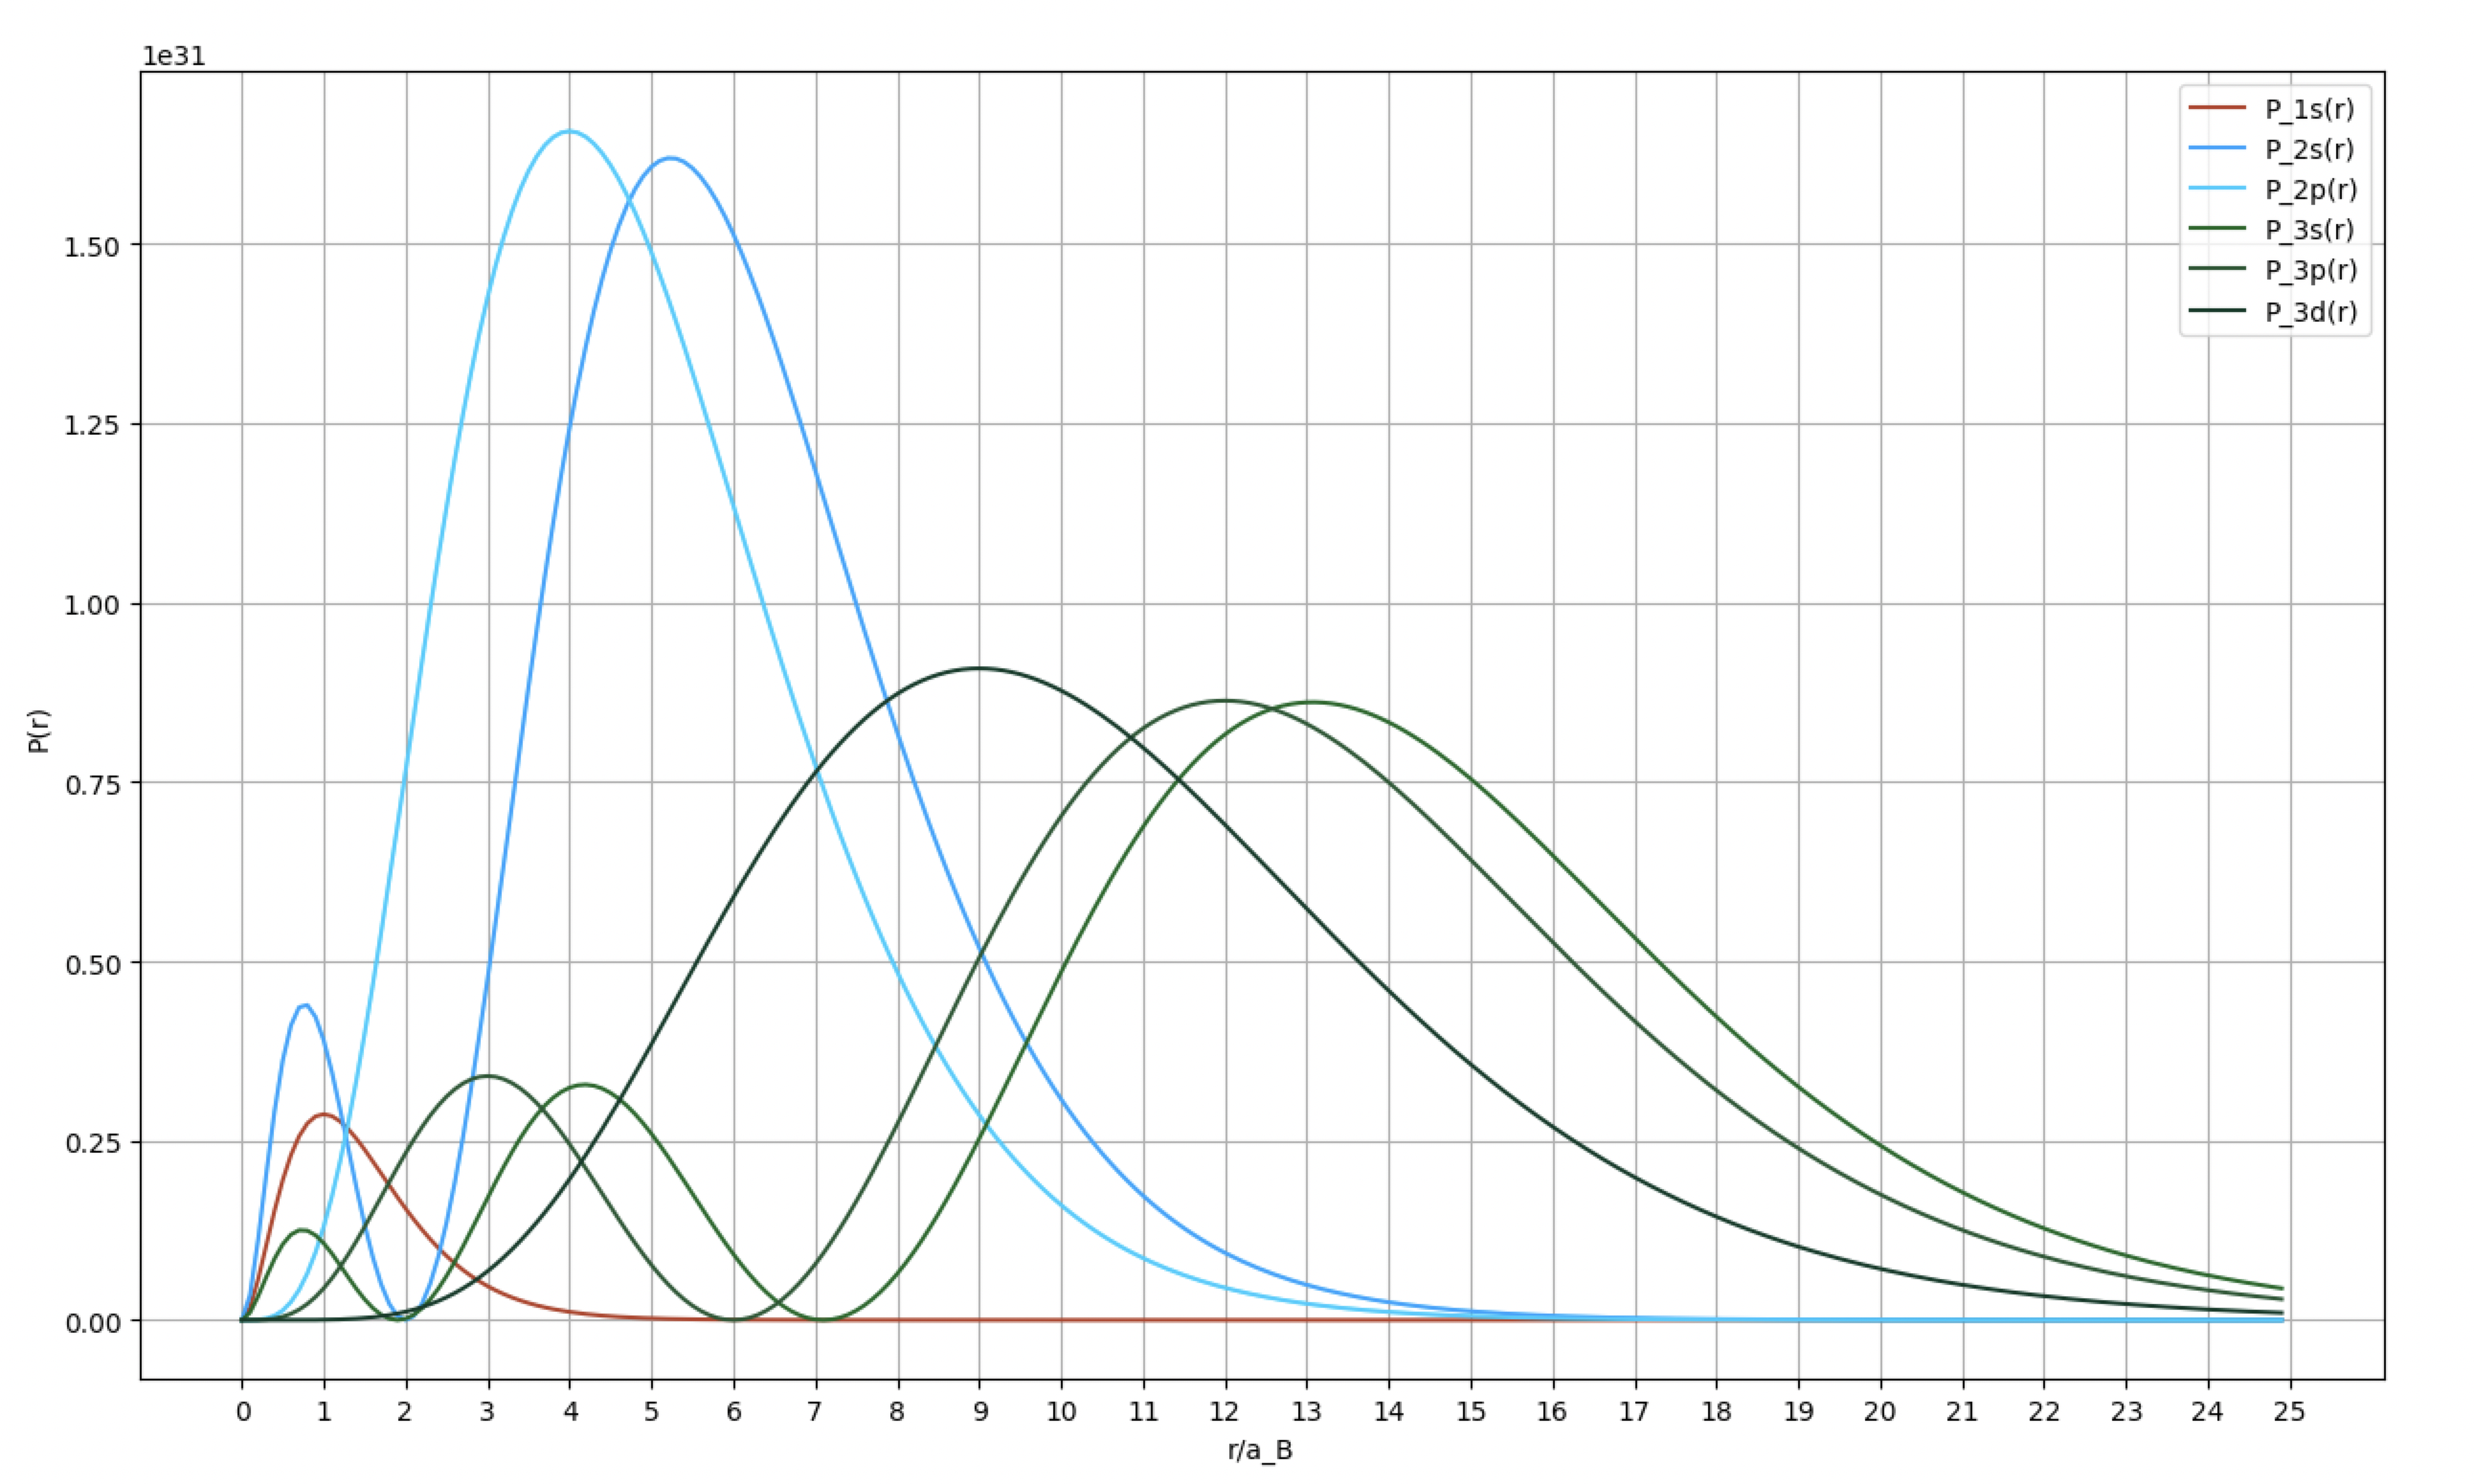
\includegraphics[scale=0.3]{ch8-8.55.png}
\end{center}
\end{proof}

\cleardoublepage
\begin{proof}{\textbf{8.56}}\\
Let us define $\rho = r/a_B$ then the radial probability distribution equation
becomes
\begin{align*}
    P(r) = \frac{4 K^3r^2}{a_B^3} e^{-2 Kr/a_B}
    = \frac{4 K^3}{a_B}\rho^2 e^{-2 K\rho}
\end{align*}
Using this formula we show below the radial probability distribution for
Hydrogen and $\text{He}^{+}$
\begin{center}
    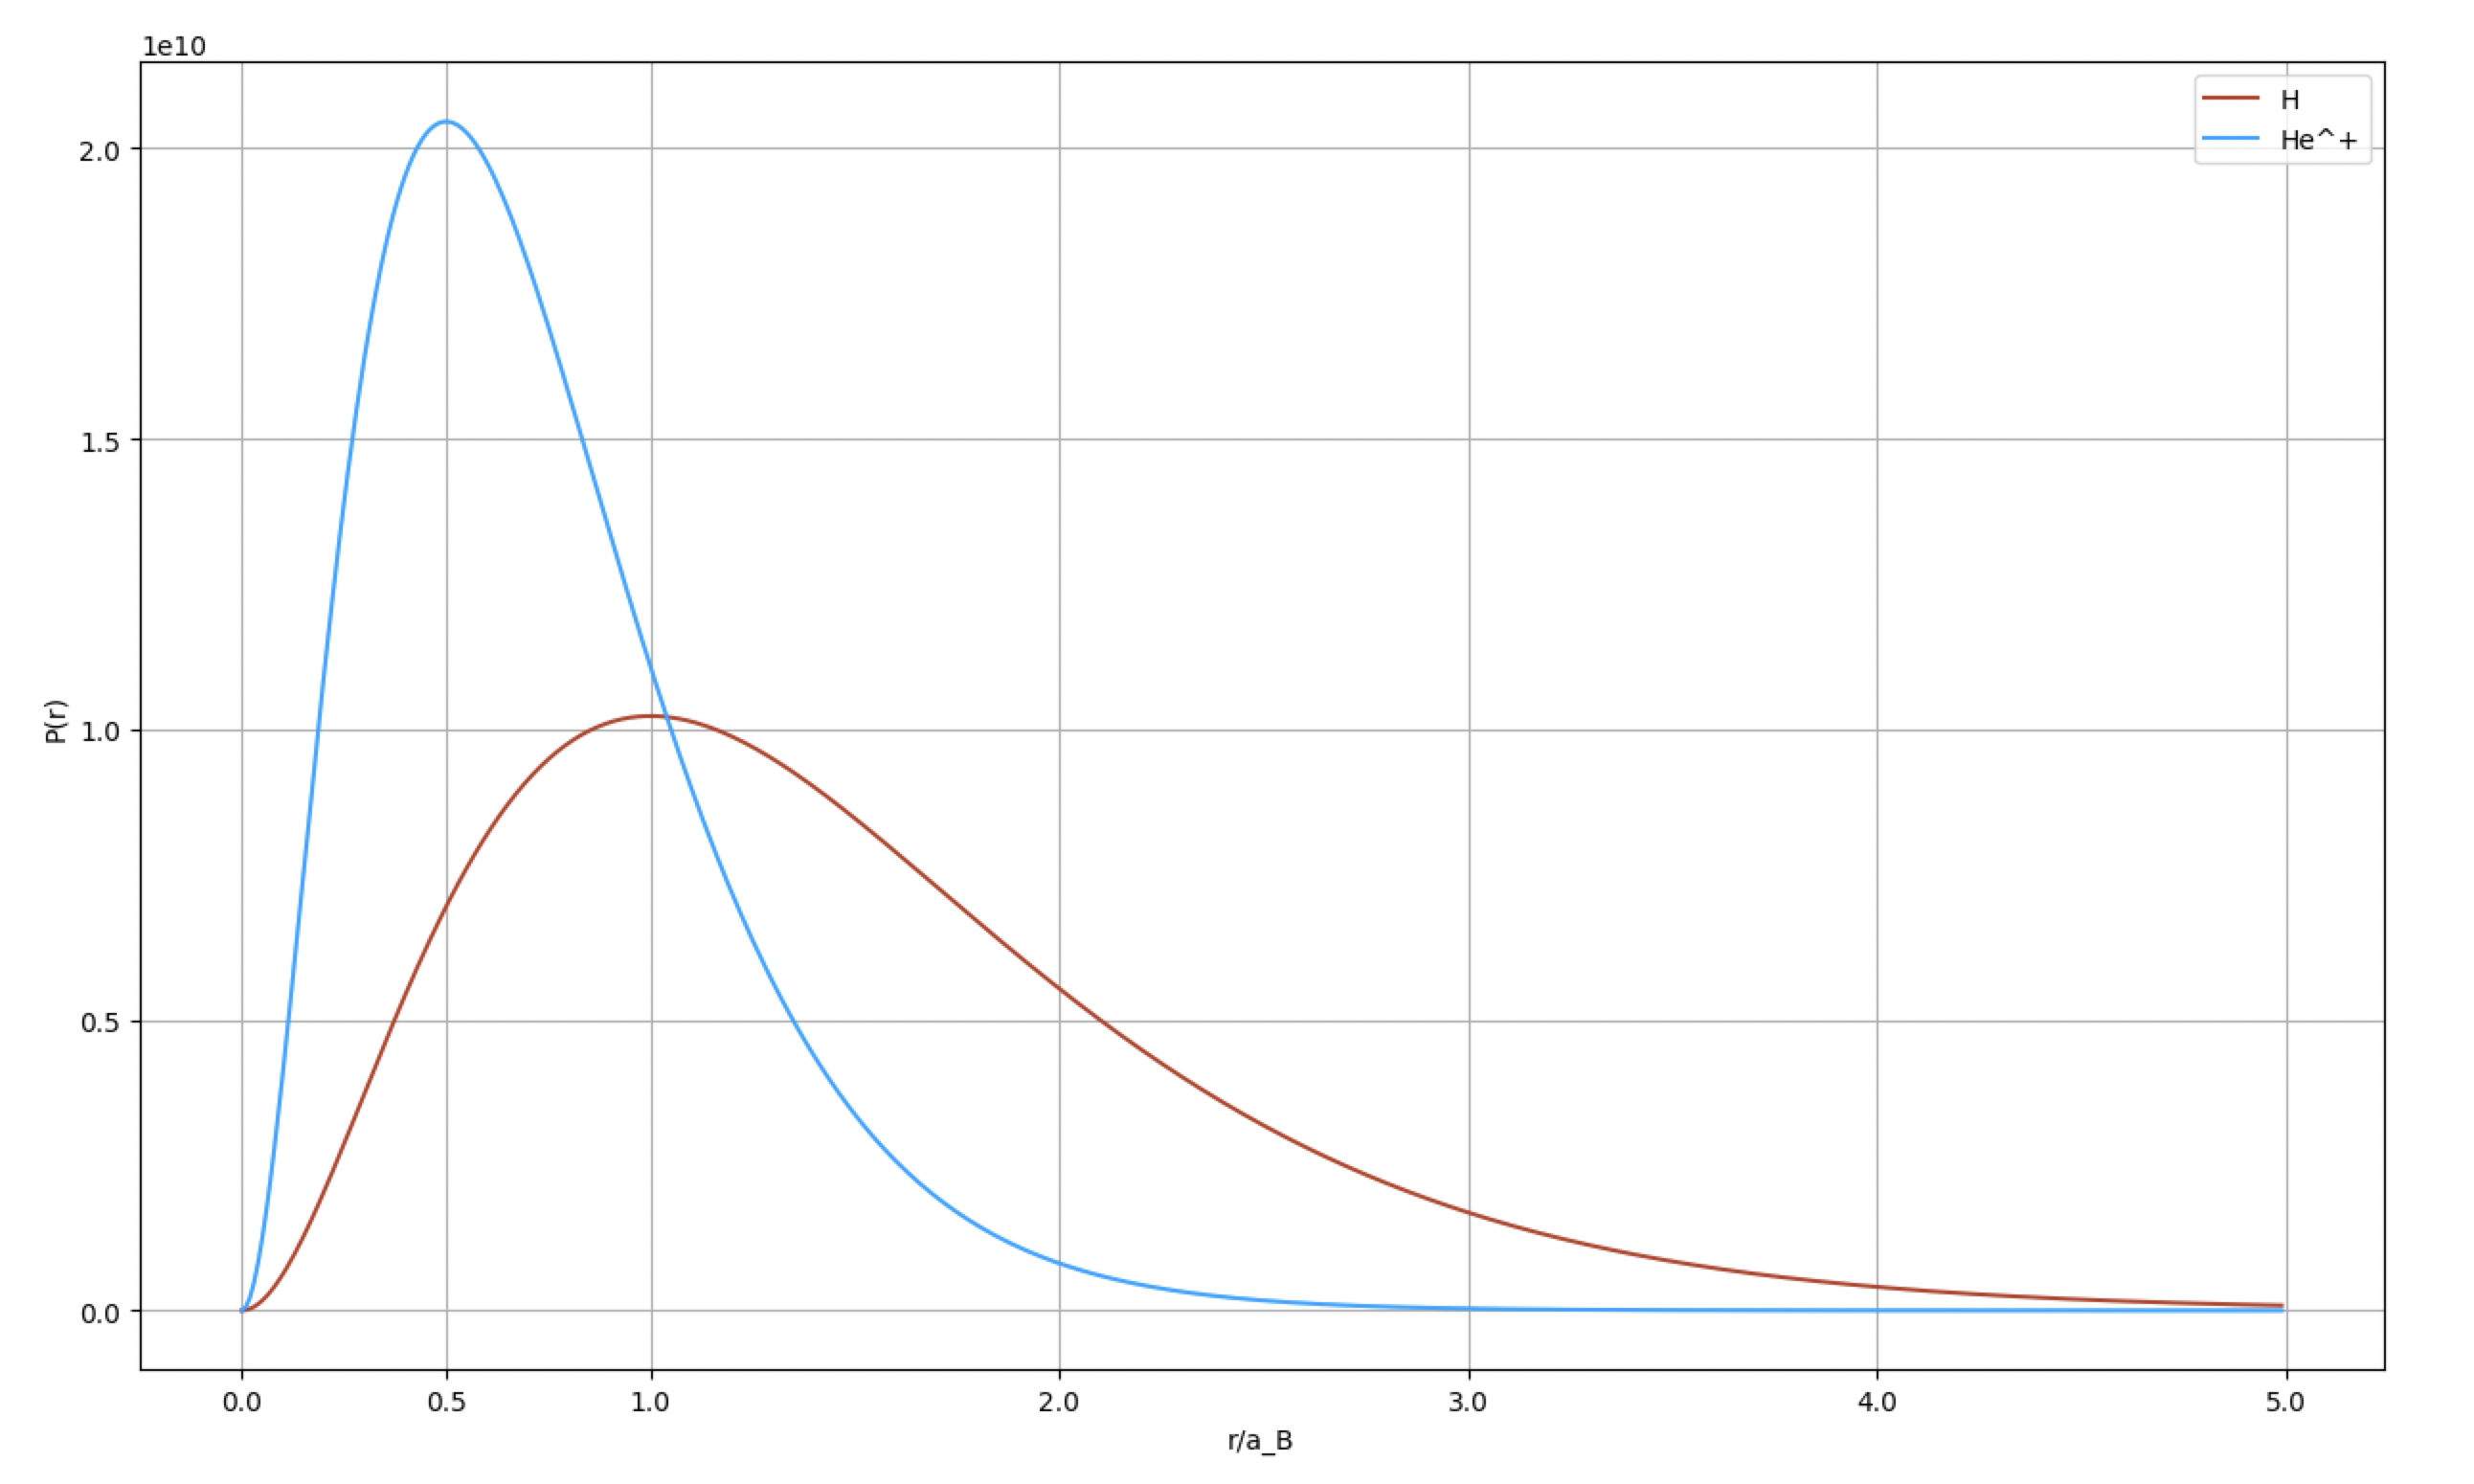
\includegraphics[scale=0.3]{ch8-8.56.png}
\end{center}
\end{proof}

\cleardoublepage
\begin{proof}{\textbf{8.57}}
\begin{itemize}
\item [\textbf{(a)}] Let us write equation (8.65) when $m = 0$ and $l = 2$
\begin{align*}
    \frac{1}{\sin\theta}\dv{\theta}(\sin\theta \dv{\Theta}{\theta})
    + 6\Theta &= 0\\
    \dv[2]{\Theta}{\theta} + \cot\theta\dv{\Theta}{\theta} + 6\Theta &= 0
\end{align*}
We can solve the equation numerically by applying the Runge-Kutta method, doing
the following replacement. Let $u = \dv{\Theta}{\theta}$ then we get the
following system of equations
\begin{align*}
    \dv{\Theta}{\theta} &= u
    \quad\text{and}\quad
    \dv{u}{\theta} = - u\cot\theta - 6\Theta
\end{align*}
Then for the case $\Theta(\pi/2) = 1$ and $\Theta'(\pi/2) = 0$ we get that
\begin{center}
    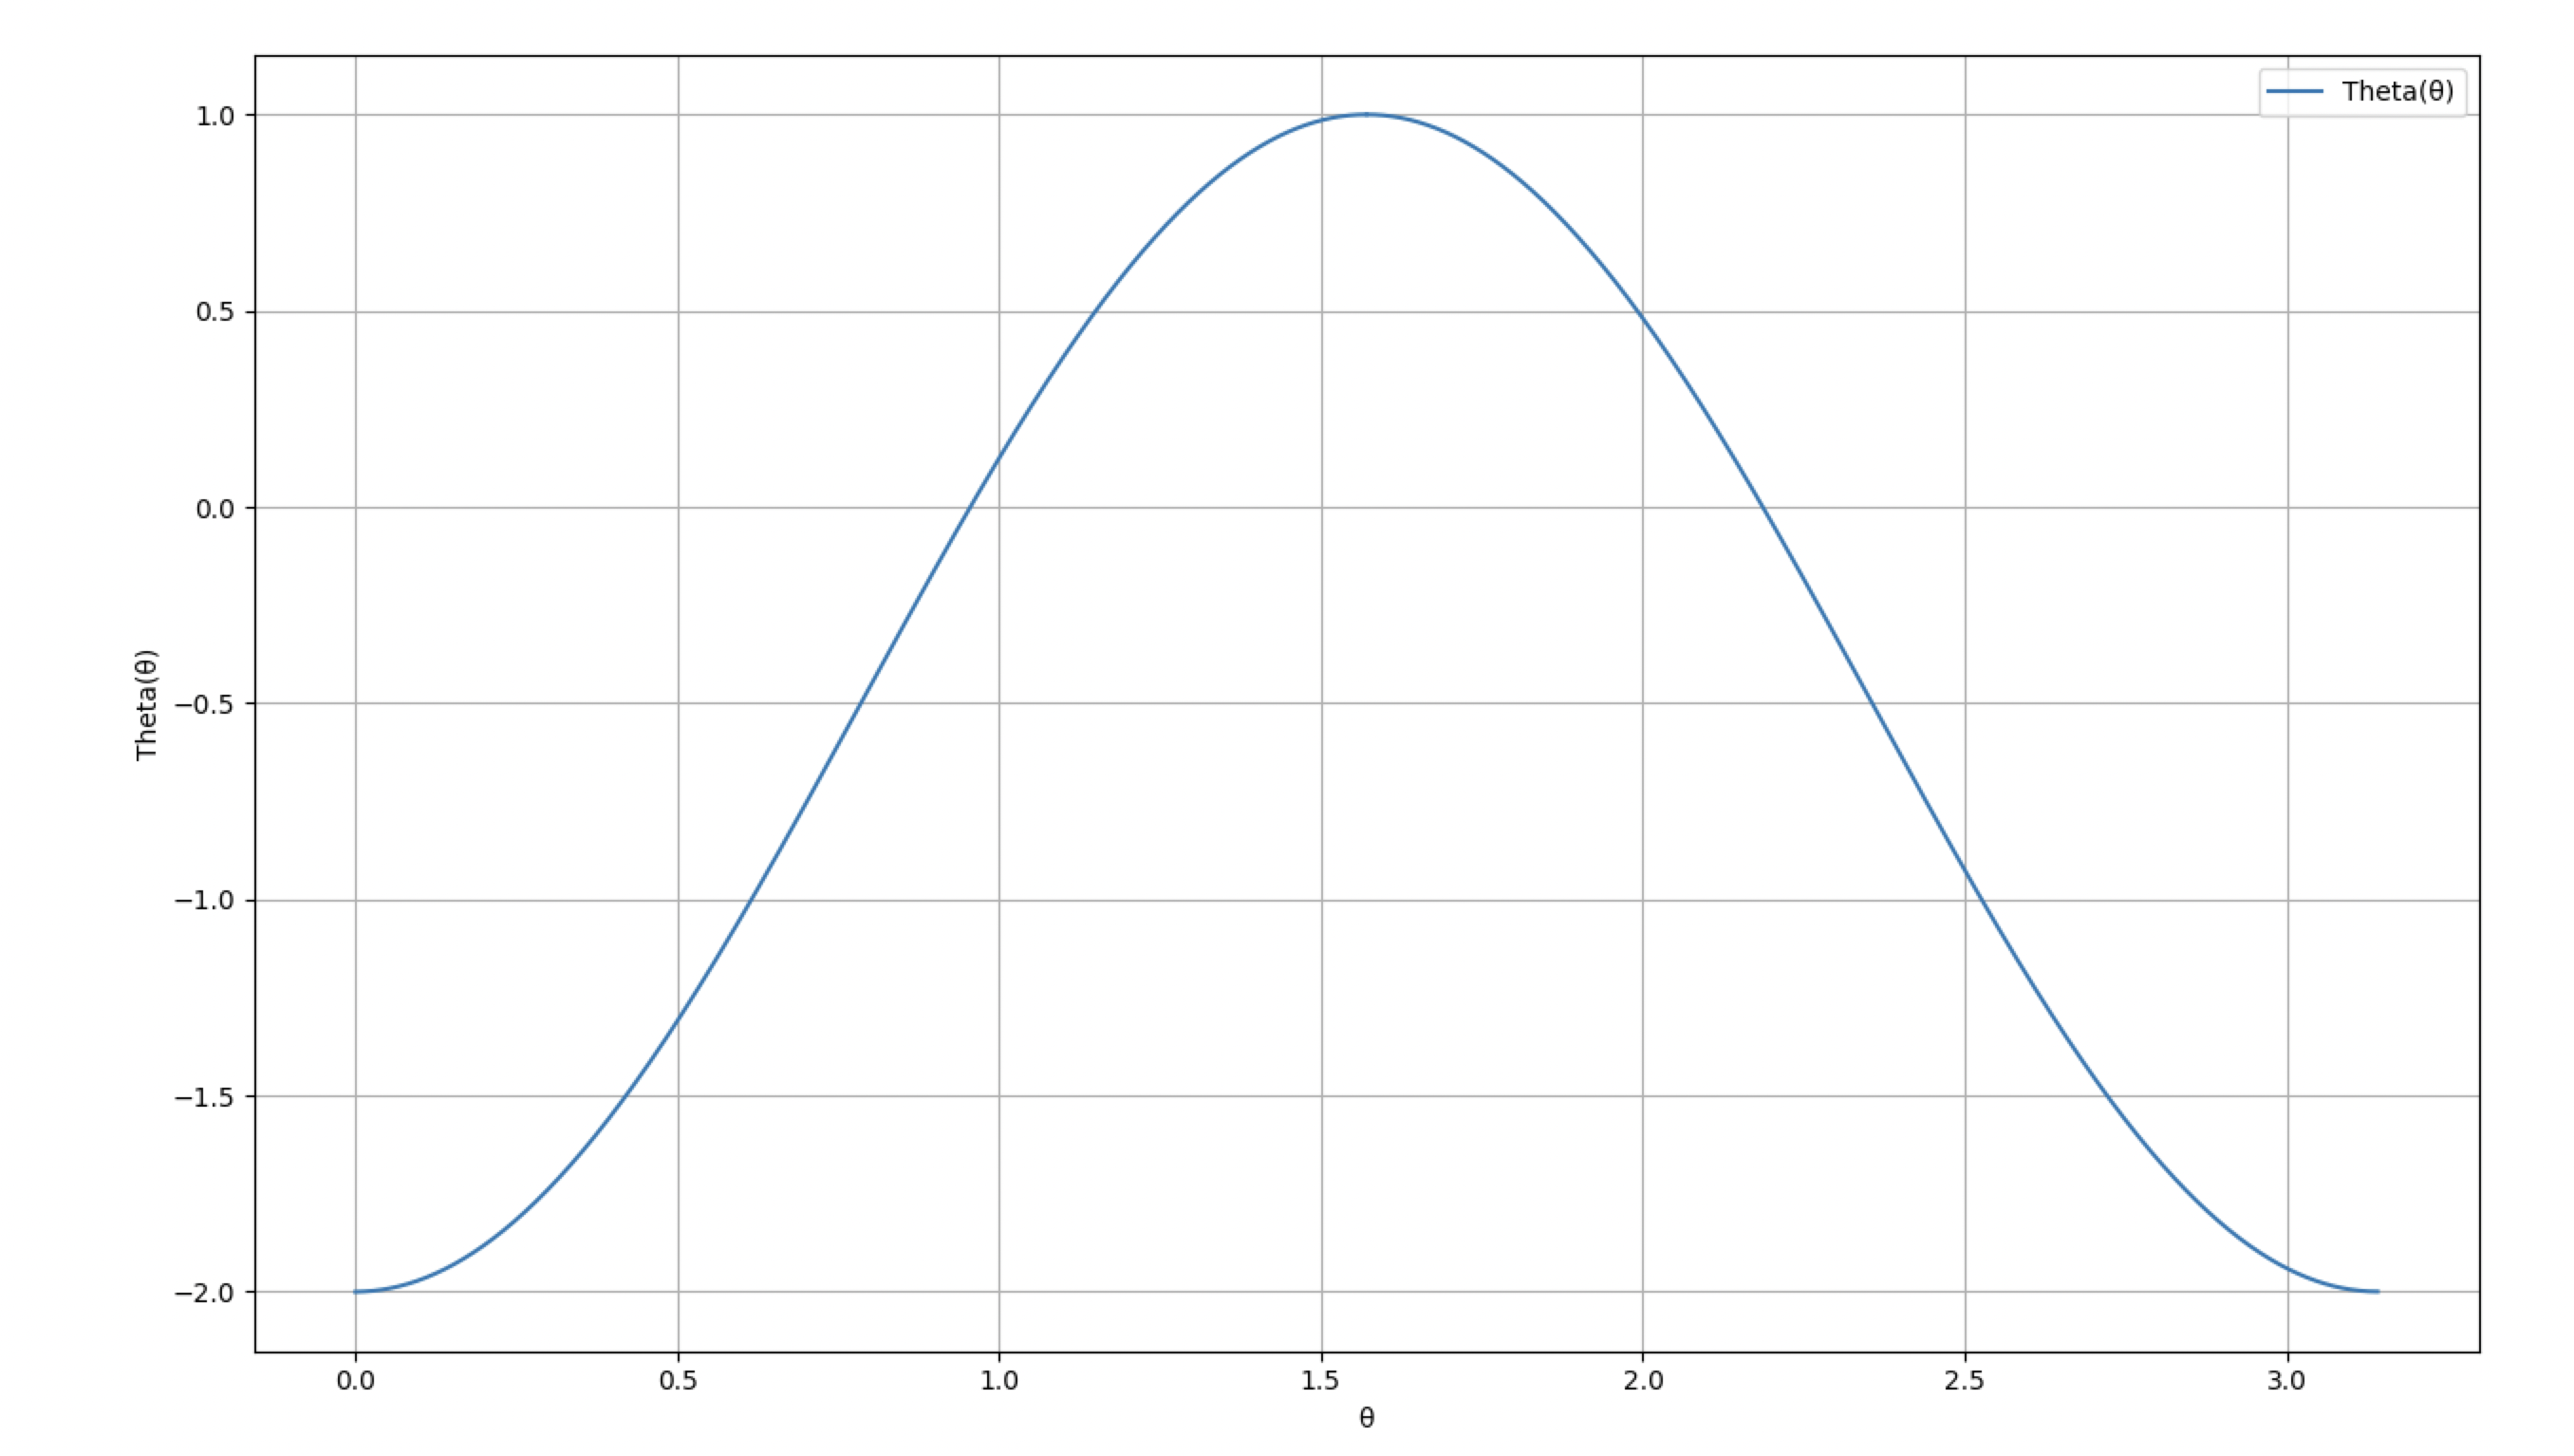
\includegraphics[scale=0.27]{ch8_8.57a.png}
\end{center}

\cleardoublepage
For the case $\Theta(\pi/2) = 0$ and $\Theta'(\pi/2) = 1$ we get that
\begin{center}
    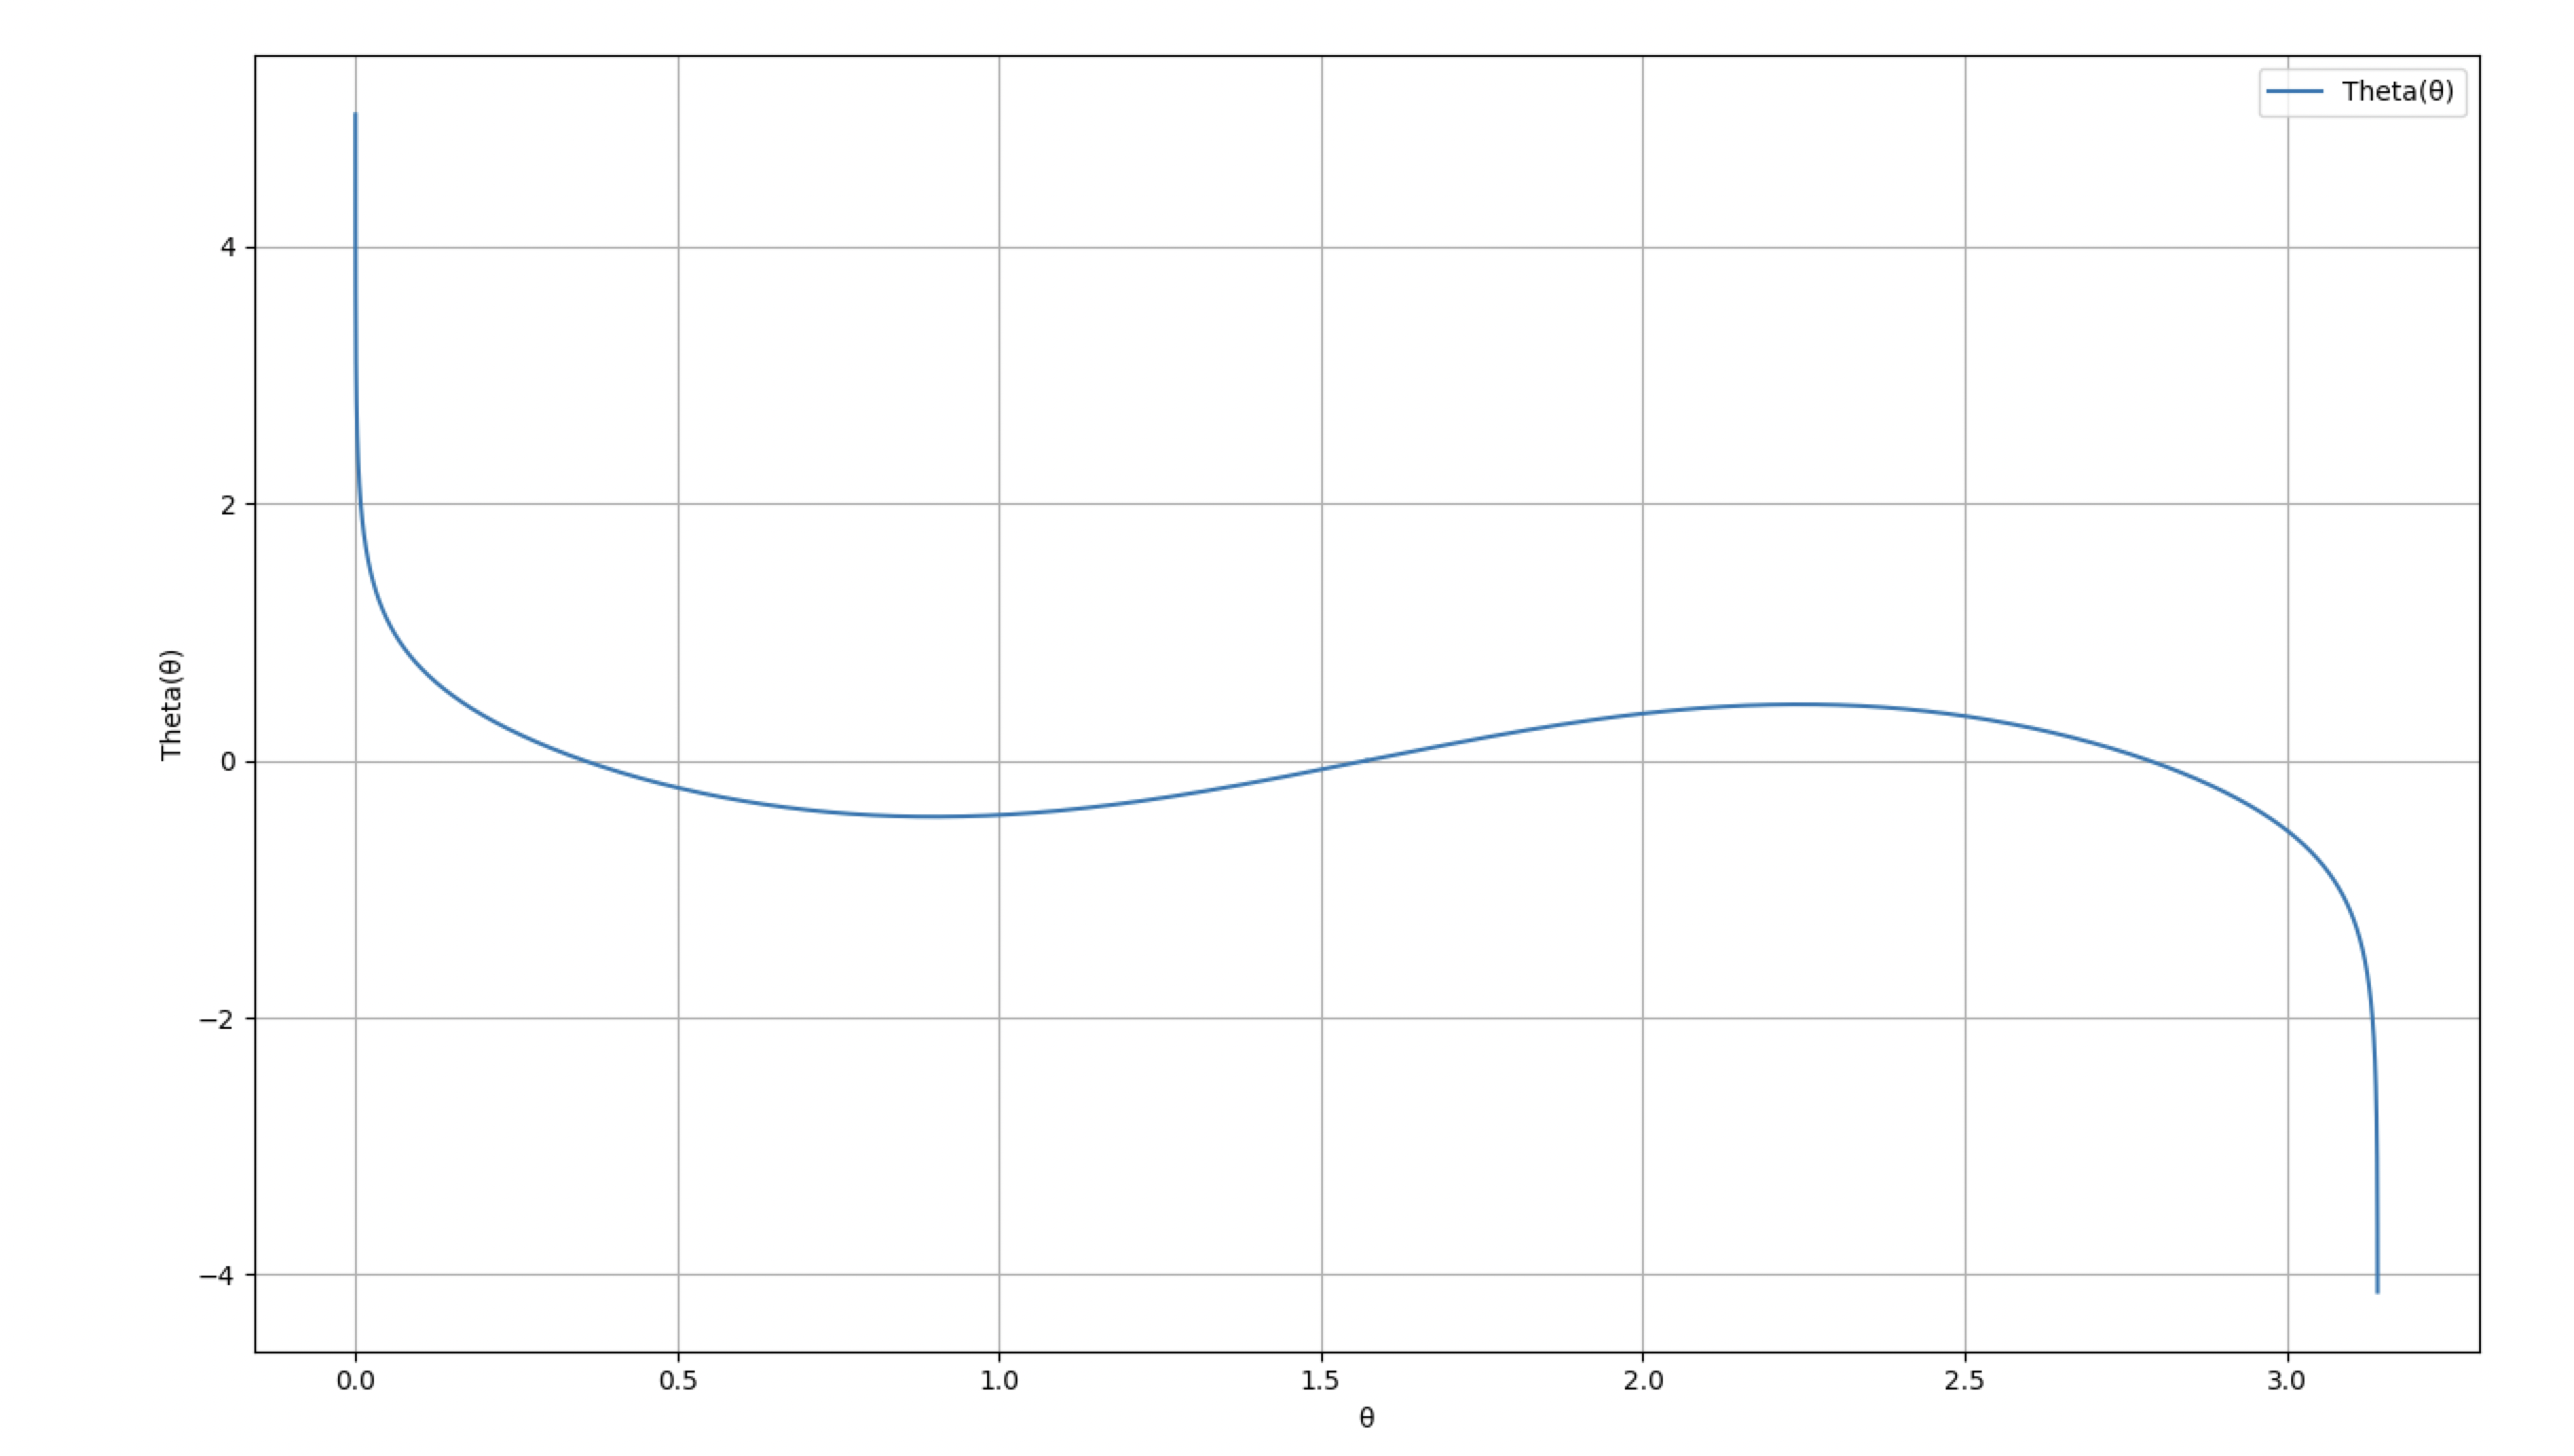
\includegraphics[scale=0.27]{ch8_8.57a2.png}
\end{center}
We see that this solution seems unacceptable because $\Theta$ at $\pi$ and 0
seems to go to infinity.

\item [\textbf{(b)}] Let us write equation (8.65) when $m = 0$ and $l = 1.75$
\begin{align*}
    \dv[2]{\Theta}{\theta} + \cot\theta\dv{\Theta}{\theta} + 4.812\cdot\Theta &= 0
\end{align*}
Then solving by Runge-Kutta for the initial conditions $\Theta(\pi/2) = 1$ and
$\Theta'(\pi/2) = 0$ we get that
\begin{center}
    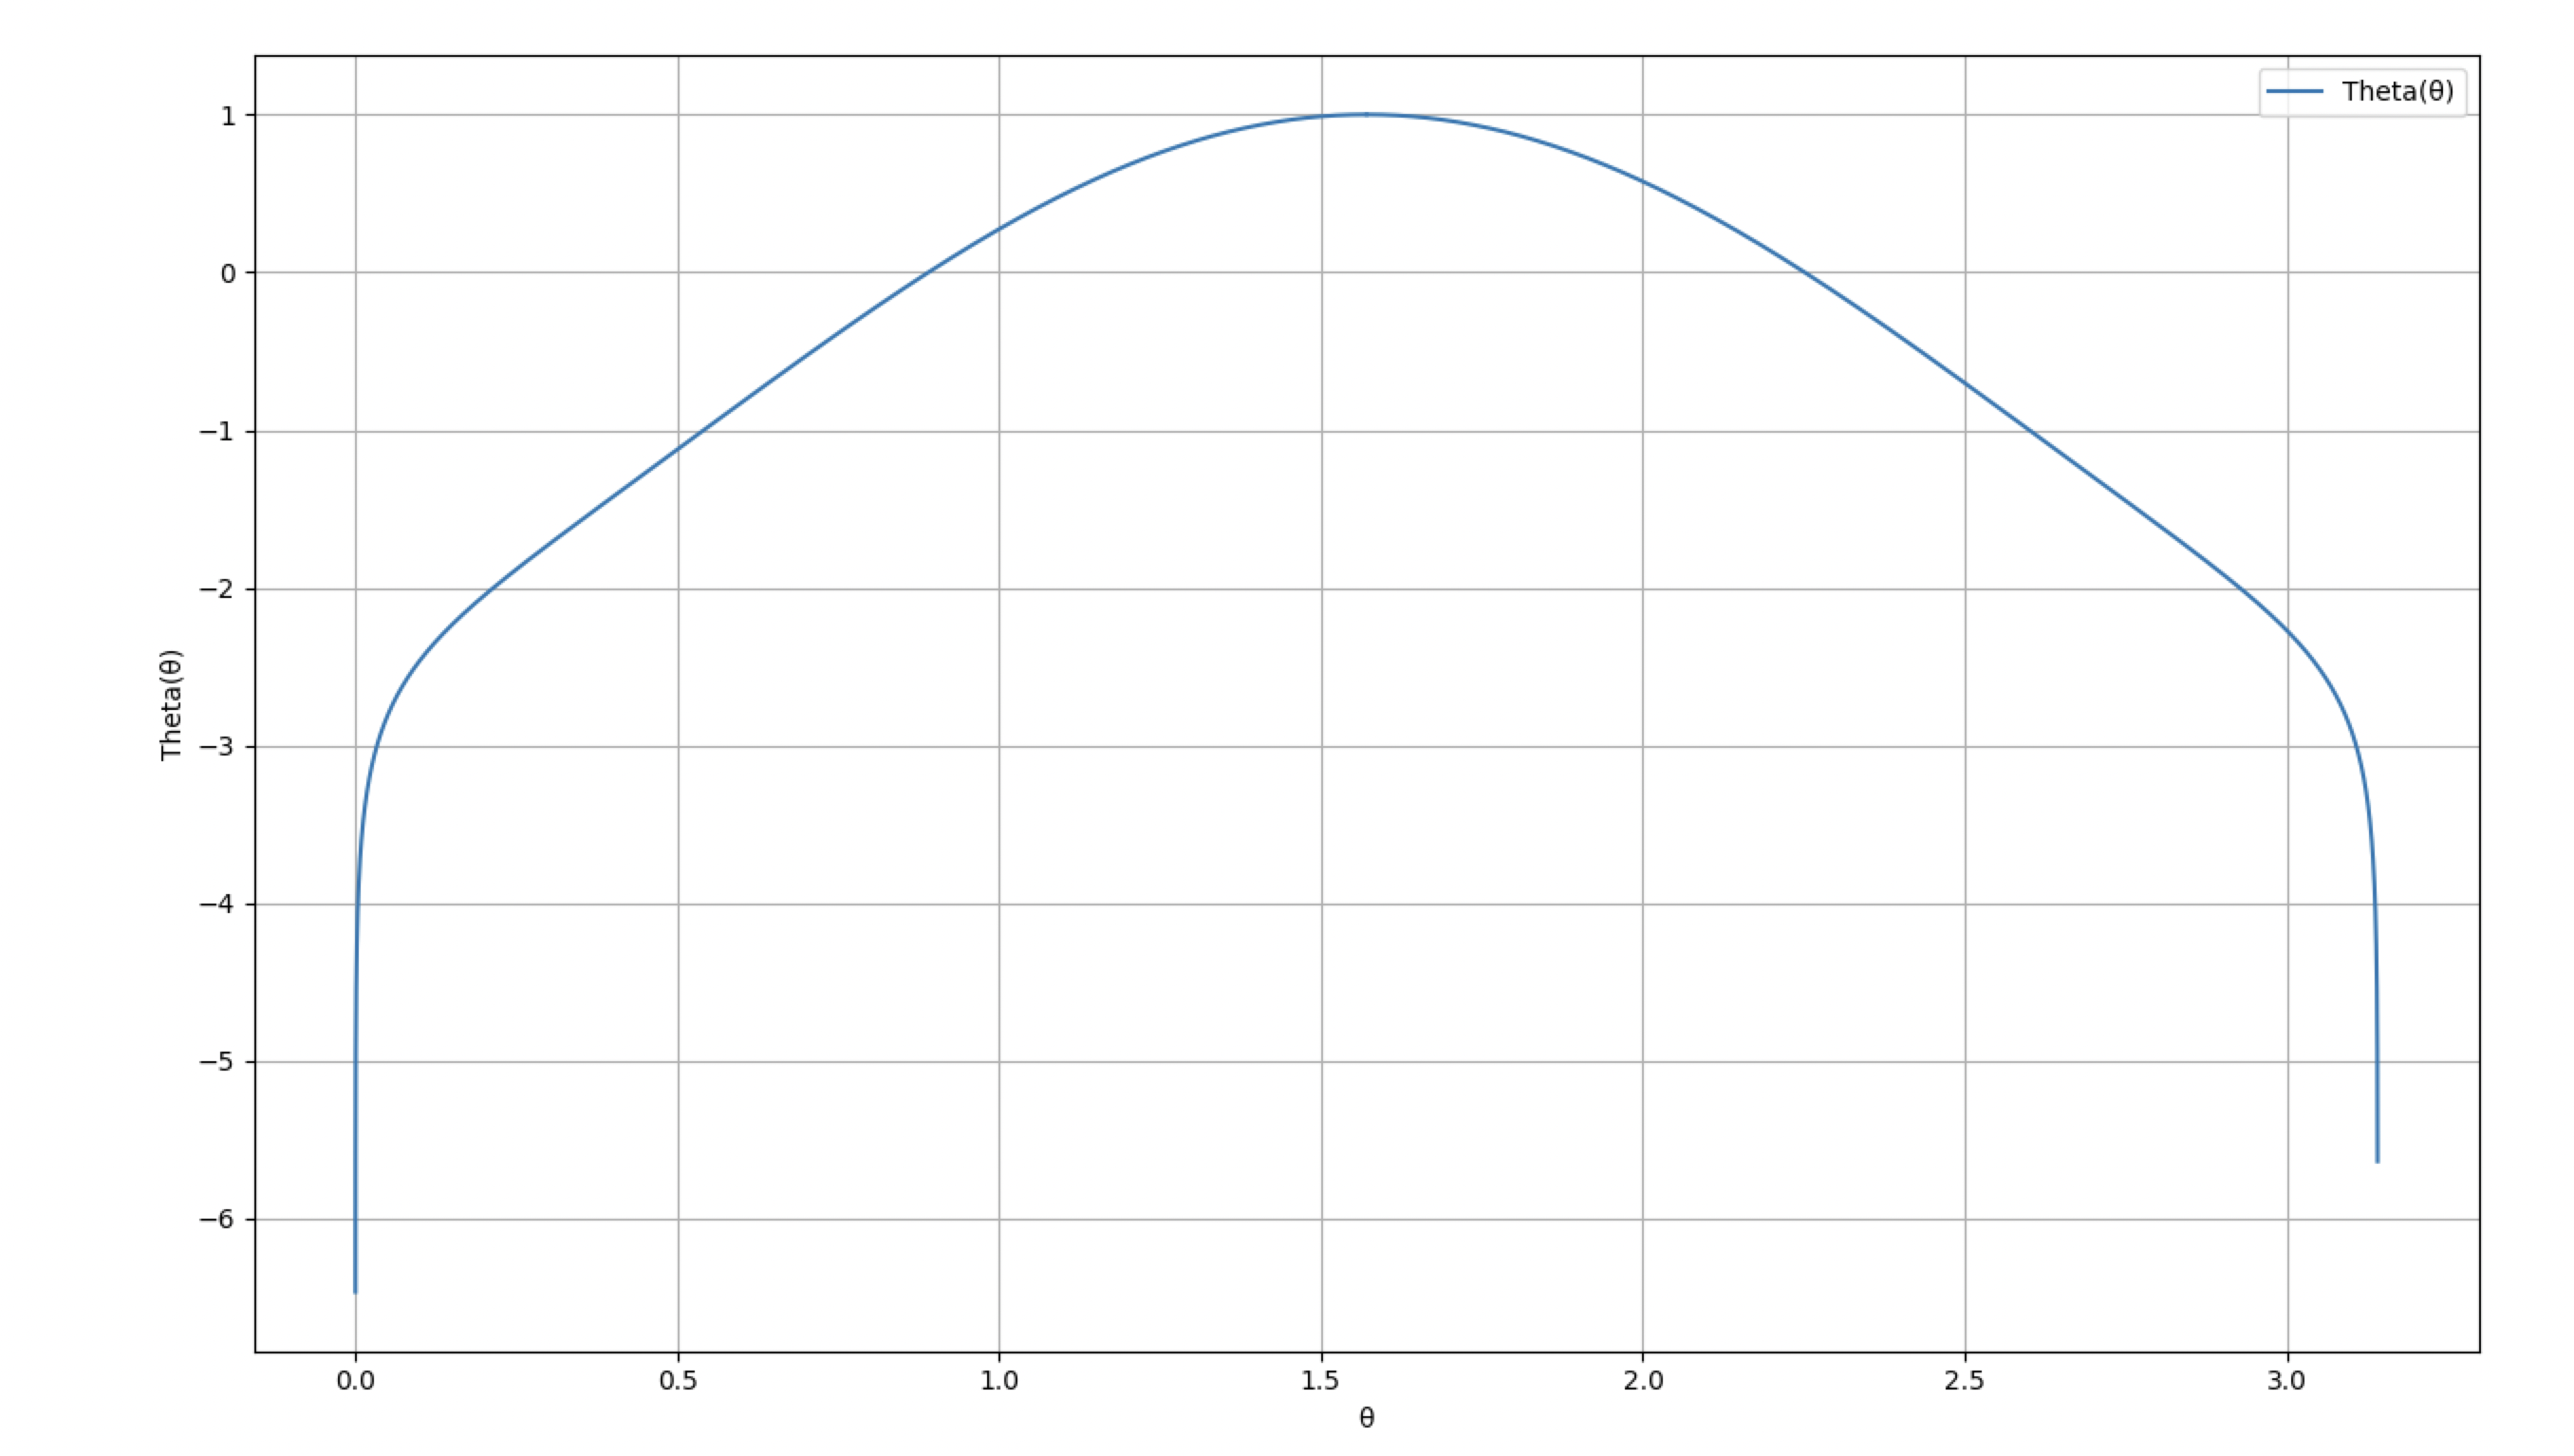
\includegraphics[scale=0.27]{ch8_8.57b.png}
\end{center}
And for the initial conditions $\Theta(\pi/2) = 0$ and $\Theta'(\pi/2) = 1$
we get that
\begin{center}
    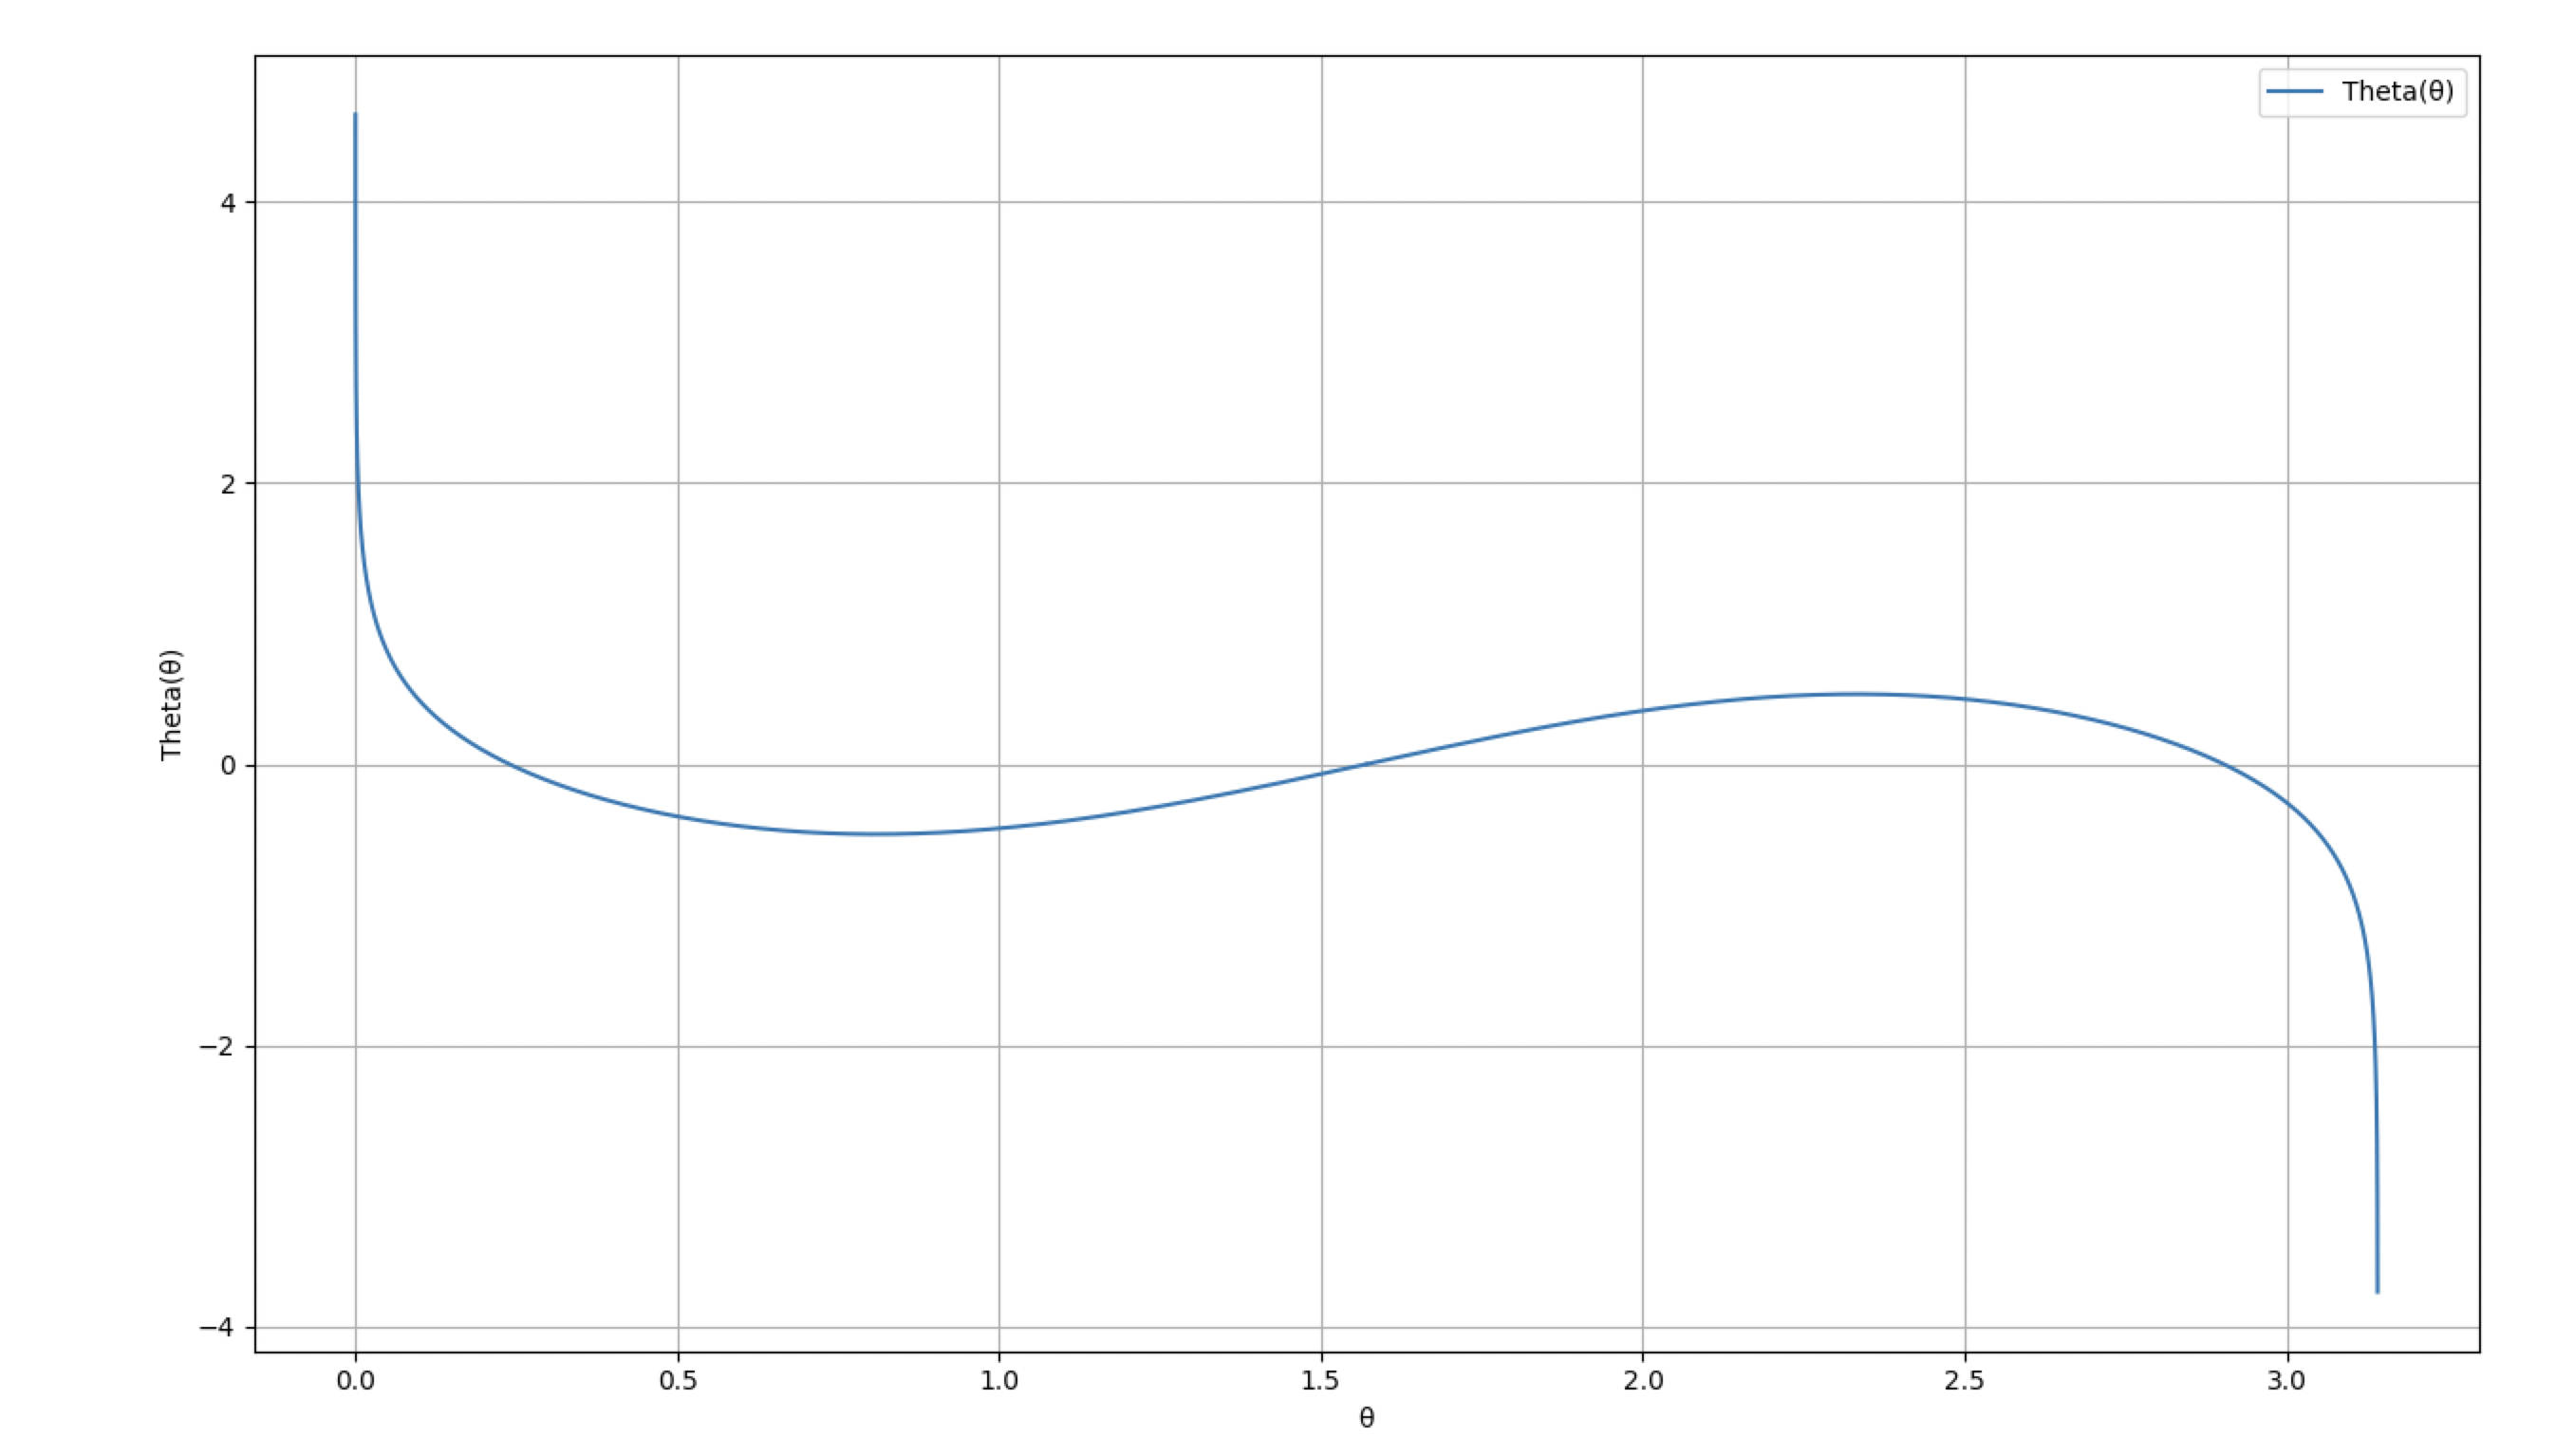
\includegraphics[scale=0.27]{ch8_8.57b2.png}
\end{center}
In both cases the solution seems to diverge as $\theta \to \pi$ and as
$\theta \to 0$.
\end{itemize}
\end{proof}

\end{document}